%% LyX 2.1.4 created this file.  For more info, see http://www.lyx.org/.
%% Do not edit unless you really know what you are doing.
\documentclass[a4paper,czech,english,12pt,a4paper,czech,english]{report}
\usepackage[cp1250]{inputenc}
\setcounter{secnumdepth}{3}
\setcounter{tocdepth}{3}
\usepackage{color}
\usepackage{babel}
\usepackage{verbatim}
\usepackage{prettyref}
\usepackage{float}
\usepackage{wrapfig}
\usepackage{calc}
\usepackage{units}
\usepackage{textcomp}
\usepackage{url}
\usepackage{amsmath}
\usepackage{amssymb}
\usepackage{graphicx}
\usepackage{esint}
\usepackage{nomencl}
% the following is useful when we have the old nomencl.sty package
\providecommand{\printnomenclature}{\printglossary}
\providecommand{\makenomenclature}{\makeglossary}
\makenomenclature
\usepackage[unicode=true,
 bookmarks=true,bookmarksnumbered=false,bookmarksopen=false,
 breaklinks=false,pdfborder={0 0 1},backref=false,colorlinks=false]
 {hyperref}
\hypersetup{pdftitle={Optimization of operation of renewable electric energy sources based on fuel cells, accumulators and PV panels for small powers},
 pdfauthor={Martin Hole�ek}}

\makeatletter

%%%%%%%%%%%%%%%%%%%%%%%%%%%%%% LyX specific LaTeX commands.
\pdfpageheight\paperheight
\pdfpagewidth\paperwidth

%% Because html converters don't know tabularnewline
\providecommand{\tabularnewline}{\\}
%% A simple dot to overcome graphicx limitations
\newcommand{\lyxdot}{.}


%%%%%%%%%%%%%%%%%%%%%%%%%%%%%% User specified LaTeX commands.
\setlength{\textwidth}{145mm}
\setlength{\textheight}{247mm}
\setlength{\oddsidemargin}{15mm}
\setlength{\evensidemargin}{15mm}
\setlength{\topmargin}{0mm}
\setlength{\headsep}{0mm}
\setlength{\headheight}{0mm}
\let\openright=\clearpage
%\ifx\uv\undefined\newcommand{\uv}[1]{,,#1``}\fi
\usepackage{amsthm,amsmath,amssymb,amscd,mathrsfs,url}
%\usepackage[czech]{babel}
%\usepackage[utf8]{inputenc}
\usepackage[cp1250]{inputenc}
\usepackage{verbatim}
%\usepackage{ictamxs}
\usepackage{showkeys}
\usepackage{xcolor}
\usepackage{stackengine}
\usepackage{lipsum}
\usepackage{comment}
%%\usepackage{MNsymbol} NIKDY!
\usepackage{graphicx}
\usepackage{caption}
\usepackage{nomencl}
\usepackage{subcaption}
\usepackage{tikz}
\usepackage[customcolors,shade]{hf-tikz}
\usepackage{marginnote}
\usepackage{esint}
\usepackage{ulem}
\usepackage{multicol}%%% v�cesloupcov� sazba
\usepackage{fancybox}%%% vkl�d�n� obr�zk�
\usepackage{psfrag}
\usepackage{fancyvrb}
\usepackage{bbding}
\usepackage{comment}
\usepackage{epstopdf} 
\usepackage{url}
\usepackage{natbib}
\DeclareGraphicsExtensions{.pdf,.eps,.png,.jpg,.mps}

%\setcounter{secnumdepth}{0}

\numberwithin{table}{chapter}
\numberwithin{figure}{chapter}
\numberwithin{equation}{chapter}

\renewcommand\[{\begin{equation}} 
\renewcommand\]{\end{equation}}

\newcommand{\opdiv}{\mathop{\mathrm{div}}}
\newcommand{\oprot}{\mathop{\mathrm{rot}}}

\newcommand{\FIGDIR}{./Obrazky}    %%% cesta do adresare s obrazky

\newcounter{definice}
\numberwithin{definice}{chapter}
\renewcommand{\thedefinice}{\arabic{chapter}.\arabic{definice}}
\newenvironment{definice}[1][]{
  \refstepcounter{definice}
  \par\medskip\noindent
  \textbf{Definice \thedefinice #1}.
}{
}

\newcounter{veta}
\numberwithin{veta}{chapter}
\renewcommand{\theveta}{\arabic{chapter}.\arabic{veta}}
\newenvironment{veta}[1][]{
  \refstepcounter{veta}
  \par\medskip\noindent
  \textbf{V�ta \theveta #1}.
  \itshape
}{
}

\newenvironment{dukaz}{
  \par\medskip\noindent
  \textit{D�kaz}.
}{
\newline
\rightline{\SquareCastShadowBottomRight}
}


\DefineVerbatimEnvironment{PCinout}{Verbatim}{fontsize=\small, frame=lines}
\DefineVerbatimEnvironment{PCinoutsmaller}{Verbatim}{fontsize=\smaller, frame=lines}

\newcommand{\Real}{\mathbb{R}}
\newcommand{\Natu}{\mathbb{N}}

\DeclareMathOperator{\Prob}{\textsf{P}}
\DeclareMathOperator{\EV}{\textsf{E}}
\DeclareMathOperator{\var}{\textrm{var}}
\DeclareMathOperator{\sd}{\textrm{sd}}

\newcommand{\betab}{\boldsymbol{\beta}}
\newcommand{\thetab}{\boldsymbol{\theta}}
\newcommand{\varepsilonb}{\boldsymbol{\varepsilon}}

\newcommand{\xb}{\boldsymbol{x}}
\newcommand{\yb}{\boldsymbol{y}}
\newcommand{\Xb}{\boldsymbol{X}}
\newcommand{\Yb}{\boldsymbol{Y}}

\newcommand{\Xm}{\mathbb{X}}

\renewcommand{\t}[1]{#1^\top}  
\bibliographystyle{alpha}
\usepackage{ae}
%\hyphenation{troj-�-hel-n�k nic-m�-n� p�ed-in-te-gro-v�-n� p��-pa-d� p�e-cho-do-v� uva-�o-va-n� na-p��-klad na-po-��-ta-nou po-�a-du-je-me umo�-n�-me mat-lab-u}
\makenomenclature

\makeatother

\begin{document}
\selectlanguage{czech}%
\pagestyle{empty} 

\begin{center}
{\large{}Charles University in Prague}
\par\end{center}{\large \par}

\begin{center}
\medskip{}
{\large{}Faculty of Mathematics and Physics}
\par\end{center}{\large \par}

\begin{center}
\vfill{}
\textbf{\Large{}MASTER THESIS}
\par\end{center}{\Large \par}

\begin{center}
\vfill{}
\centerline{\mbox{
\includegraphics[width=60mm]{Obrazky/logo}}}
\par\end{center}

\begin{center}
\vfill{}
\vspace{5mm}

\par\end{center}

\begin{center}
{\LARGE{}Martin Hole�ek}
\par\end{center}{\LARGE \par}

\begin{center}
\vspace{15mm}

\par\end{center}

\begin{center}
\textbf{\LARGE{}Optimization of operation of renewable electric energy
sources based on fuel cells, accumulators and FV panels for small
powers}
\par\end{center}{\LARGE \par}

\begin{center}
\vfill{}
Mathematical Institute of Charles University
\par\end{center}

\begin{center}
\vfill{}

\par\end{center}

\begin{center}
\begin{tabular}{rl}
Supervisor of the master thesis: & prof. Ing. Franti�ek Mar��k, DrSc.\tabularnewline
%% Jm�no a p��jmen� s~tituly \\
\noalign{\vspace{2mm}
} Study programme:  & Mathematics\tabularnewline
\noalign{\vspace{2mm}
} Specialization: & Mathematical Modelling in Physics and Technology\tabularnewline
\end{tabular}
\par\end{center}

\begin{center}
\vfill{}

\par\end{center}

\begin{center}
% Zde doplnte rok
Prague 2015%%% N�sleduje vev�zan� list -- kopie podepsan�ho "Zad�n� diplomove pr�ce".
%%% Toto zad�n� NEN� sou��st� elektronick� verze pr�ce, nescanovat.
%%% Na tomto m�st� mohou b�t naps�na p��padn� pod�kov�n� (vedouc�mu pr�ce,
%%% konzultantovi, tomu, kdo zap�j�il software, literaturu apod.)
\newpage{}\openright
\par\end{center}

D�kuji panu profesorovi Mar��kovi za podporu p�i vypracov�n� a zkontaktov�n�
s v�zkumn�mi kolegy a panu Douckovi za vzorov� data pro testov�n�.

\noindent %%DOD: D�kuji panu Hronovi za podporu a pomoc v .
%%% Strana s �estn�m prohl�en�m k diplo pr�ci
\newpage{}\vglue 0pt plus 1fill

\noindent I declare that I carried out this master thesis independently, and only with the cited sources, literature and other professional sources.

\medskip\noindent

I understand that my work relates to the rights and obligations under the Act No.~121/2000 Coll., the Copyright Act, as amended, in particular the fact that the Charles University in Prague has the right to conclude a license agreement on the use of this work as a school work pursuant to Section 60 paragraph 1 of the Copyright Act.

\vspace{10mm}

\hbox{
  \hbox to 0.5\hsize{
  In ........ date ............ 
\hss
}
\hbox to 0.5\hsize{
  signature of the author 
\hss
}
}
\vspace{20mm}

\newpage{}

\vbox to 0.5 \vsize{\setlength{\parindent}{0mm}\setlength{\parskip}{5mm}

N�zev pr�ce: Optimalizace funkce obnoviteln�ch zdroj� elektrick� energie
na b�zi palivov�ch �l�nk�, akumul�tor� a FV panel� pro mal� v�kony.

Autor: Martin Hole�ek

Katedra: Matematick� �stav UK

Vedouc� diplomov� pr�ce: prof. Ing. Franti�ek Mar��k, DrSc., Matematick�
�stav UK %% Jm�no a p��jmen� s tituly, pracovi�t�
%% dle Organiza�n� struktury MFF UK, p��padn� pln� n�zev pracovi�t� mimo MFF UK


Abstrakt: 

Prvn� ��st pr�ce je v�novan� hlub�� re�er�i do literatury optim�ln�ho
��zen�, shrnut� princip� a zp�sob� jak je aplikovat na prezentovan�
probl�m. N�sledn� je sestaven a pops�n model pou�iteln� pro samostatnou
energetickou jednotku s~pou�it�m vod�kov�ch �l�nk�, akumul�toru a
fotovoltaick�ch panel�, spolu s~nej�ast�j��mi pou��van�mi rovnicemi
z literatury. Tak� je formulov�n probl�m optim�ln�ho ��zen� �e�en�ho
syst�mu pro optim�ln� cenu v~provozu p�i nejlep��ch podm�nk�ch. D�le
jsou pops�ny algoritmy numerick�ho �e�en� syst�mu spolu s~implementac�
konkr�tn�ho numerick�ho algoritmu ,,multiple shooting\textquotedbl{}
na tento probl�m a~ numerick� testy a v�sledky.

Kl��ov� slova: ��d�c� syst�my, palivov� �l�nky, stacion�rn� zdroje
energie

\vss}
\nobreak \vbox to 0.49 \vsize{ \setlength{\parindent}{0mm} \setlength{\parskip}{5mm}

Title: Optimization of operation of renewable electric energy sources
based on fuel cells, accumulators and FV panels for small powers.

Author: Martin Hole�ek

Department: Mathematical Institute of Charles University

Supervisor: prof. Ing. Franti�ek Mar��k, DrSc., Ph.D., Mathematical
Institute

Abstract: 

The first part of the research is motivated to provide citations deeper
to the literature of optimal control principles that could be linked
to the system optimization problem, discuss these principles and various
ways to apply them. Then we describe one fuel cell, accumulator and
photovoltaic standalone system along with the most used equations
from the literature. Next, we formulate the problem of optimal control
for this system to optimize the system financial cost in the best
case and we process to describe and discuss the numerical optimal
control algorithm - multiple shooting - that will be used to solve
the problem, that was not used in literature so far in conjunction
with the problem. The codes and numerical simulations are also provided.

Keywords: control systems, fuel cells, stationary electric energy
sources \vss}

%%% Strana s automaticky generovan�m obsahem diplol��sk� pr�ce. U matematick�ch
%%% prac� je p��pustn�, aby p��padn� seznam tabulek a zkratek, existuj�-li, byl um�st�n
%%% na za��tku pr�ce, m�sto na jej�m konci.
\newpage{}\openright
\pagestyle{plain}
\setcounter{page}{1}\tableofcontents{}\selectlanguage{english}%



\pagebreak{}\printnomenclature
\addcontentsline{toc}{chapter}{Nomenclature}\pagebreak{}


\chapter*{Motivation and introduction}

%\setcounter{chapter}{1}
\stepcounter{chapter}
\addcontentsline{toc}{chapter}{Motivation and Introduction}

For better understanding of the whole problem and work, lets imagine
a model situation, that we can follow. Lets say, we want to make an
energy independent unit - ecologic house, for example.

Lets add renewable energy source (photovoltaic panels) and a system
for storing energy. Batteries alone are not sufficient, because they
would need to be changed, due to degradation. So lets add availible
hydrogen technologies - electrolyzer, hydrogen tank, fuel cells. And,
to finish the setting, backup energy unit (or electric grid). The
goal is to determine the system parameters (and develop the strategy
to do so) and power managment strategy in a manner to make the system
independent as much as possible (minimizing the consumption of backup
energy or energy from grid).

\begin{comment}
In this work not only do we want to solve this problem, but also to
make this text usefull for future coworkers,
\end{comment}


For now, lets look at the theoretical and practical tools needed to
solve this problem in the following part ``research and previous
works''. Later we will return to our model problem, and we will use
the tools to analyze the setting and rewrite it into mathematical
formulation. 

Lastly, there will be a brief note about the developed algorithms.

\begin{comment}
At our disposition we will have (or will develop) model for the system
with equations for parts of the system and supplying datas for daily
light current and energy demand.
\end{comment}
\begin{figure}[b]
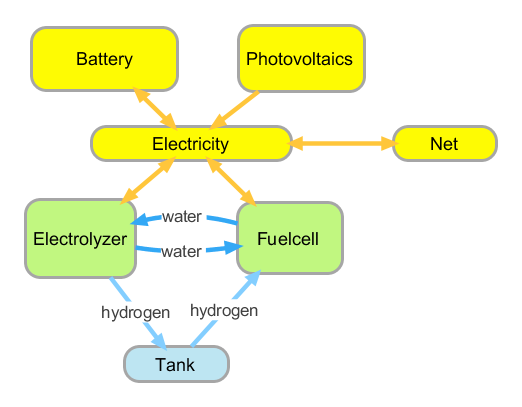
\includegraphics[width=0.45\textwidth]{Schema-copy}\includegraphics[width=0.45\textwidth]{instalace}\caption{Schema of functional units (left) and a photo of existing installation
in �JV �e� (right) \cite{UJVInst}}
\end{figure}



\chapter*{Basic assumptions and definitions}

%\setcounter{chapter}{2}
\stepcounter{chapter}
\addcontentsline{toc}{chapter}{Research and previous works}

In this section, lets look at other works and summarize concepts from
the relevant fields.


\section{Optimization and hydrogen technology}

Fuel cells and hydrogen technologies (as a part of renewable resources
\cite{RenewableSources}), extend the possibilities of energy storage
\cite{EnergyAccumulation} and create a need for deeper research of
various systems using mathematical tools to model and optimize these
systems. One example of such a system are standalone energetic units
\cite{MassimoStandalone}.

Some methods of optimization of these standalone systems are summarized
in \cite{ErdincOptimumDesign}, optimization of standalone energetic
units and power managment strategies are being researched too (in,
for example \cite{IpsakisPowerManagmentStrategies}), and some works
are also focused on specific installations \cite{Abdelkafi20141},
\cite{Sarioglu20147}, \cite{Taher2014268}, \cite{Cai2014212}. Also
optimization problems are solved for vehicles \cite{Maalej2014668}.
In the article \cite{CaliseSingleLevel}, there is proposed an optimal
system even for the powerplant of SOFC (solid oxide fuel cell \nomenclature{SOFC}{Solid oxide fuelcell})
type. Practical measurements of standalone systems efficiency are
described together with theoretical background in \cite{VyrobaAVyuziti}.

From the other side, practical application of optimization in the
theory of optimal control is described in the books \cite{EvansControlCourse},
\cite{Lewis2012optimal}, \cite{Warga1972optimal}. An example of
a method used for global optimization is an application of metropolis
algorithm, so called Simulated annealing \cite{SimulatedAnnealing}
(that was originally used for the design of electric circuits or in
chemistry \cite{Chaudhuri1997733}). There is even a method taking
in account the uncertainity of data, called Stochastic annealing \cite{PaintonStochastic}.
This method is used in \cite{GiannakoudisOptimumDesign} for optimization
of the parameters of a control strategy.

Another interesting optimization principle, the Pontryagin principle,
is used to prolong the lifetime of such systems \cite{XuPontryaginStrategy,ProlongingLifetime,ZhengPontryaginProlonging}.

Needed to say, that new algorithms of global optimization are often
being used (ex. particle swarm, or genetic algorithms). For these
algorithms, the question of convergence is still an open problem (about
this and another possibilities of such algorithms see the text \cite{ExperimentalAlgorithms}). 




\paragraph*{}


\section{Models for batteries, fuel cells, electrolyzer, photovoltaics...}

There are rich availible model descriptions (for example also in \cite{vepa2013dynamic}),
complex models (with PDEs \nomenclature{PDE}{Partial differential equation})
are used for complicated problems and for detailed desription of inside
processes (for example in a battery), but these models aren't meant
and suited for simulations taking longer time or scale. More simple
models with less variables (for example like curve fitting) are better
in case in which we do need to evaluate the model more times per run
(as in our case).


\subsection{Photovoltaics}

When looking at photovoltaic (PV \nomenclature{PV}{Photovoltaic, usually photovoltaic panels})
panels, if we want a better model than just saying ``general power
source\textquotedbl{}, we need to consider that the photoelectric
effect (the power source) happens at the P-N junction, which is, of
course, a diode, and that there is also some ressistance present.
Thats the reason, why the following (\ref{fig:5-parameter-equivalent})
equivalent circuit - ``5 parameter circuit\textquotedbl{} - is used
(there exists even the so called ``7 parameter circuit\textquotedbl{}
which has another diode in parallel to the first diode). 

\begin{wrapfigure}{O}{0.5\columnwidth}%
\includegraphics[width=0.4\textwidth]{275px-Solar_cell_equivalent_circuit\lyxdot svg}\caption{\label{fig:5-parameter-equivalent}5 parameter equivalent circuit
for photovoltaic panel}
\end{wrapfigure}%
Construction details, like material used (single crystalline silicon,
polycrystalline and semicrystalline, thin films, amorphous silicon,
spheral...) or additional tricks (concentrated cells, lens, antireflexive
and other coating) affect the parameters and the efficiency. 

The circuit supplies current $I=I_{pv}$ at voltage $V=V_{pv}$, $I_{L}$
is generated current by photovoltaic effect and from that we subtract
diode current and shunt current. This way we can derive the model:

\begin{equation}
I_{pv}=I_{L}-I_{D}-I_{sh}=I_{L}-I_{0}(\exp(\frac{V_{pv}+I_{pv}R_{s}}{\alpha}))-\frac{V_{pv}+I_{pv}R_{s}}{R_{sh}}
\end{equation}
\nomenclature{$I_{pv}$}{Current from photovoltaic model circuit ($A$)}
\begin{equation}
I_{L}=C_{1}G,\,I_{0}=C_{2}T^{3}\exp(\frac{-E_{GO}}{kT})
\end{equation}
\begin{equation}
P_{pv}=V_{pv}I_{pv}\eta_{conv}
\end{equation}
 \nomenclature{$P_{pv}$}{Power from photovoltaic model circuit ($J$)}
\begin{itemize}
\item $\alpha$ curve fitting parameter (model requires test runs and measurements)
\item $G$ incident radiation {[}$W/m^{2}${]} \nomenclature{$G$}{Incident radiation ($W/m^2$)}
\item $T$ surface temperature ($K$)
\item $E_{GO}$ band gap of the used PV material \nomenclature{$E_{GO}$}{band gap of the used PV material}
\item $C_{i}$ constants
\item $I_{L}$ light current {[}$A${]}\nomenclature{$I_L$}{light current ($A$)}
\item $I_{D}$ diode current {[}$A${]} \nomenclature{$I_{D}$}{diode current ($A$)}
\item $I_{sh}$ shunt current {[}$A${]} \nomenclature{$I_{sh}$}{shunt current ($A$)}
\item $I_{0}$ diode reverse saturation current (comes from the Shockley's
diode equation) {[}$A${]} \nomenclature{$I_{0}$}{diode reverse saturation current ($A$)}
\item $V_{pv}$, $I_{pv}$, operational voltage and current {[}$V${]},
{[}$A${]} \nomenclature{$V_{pv}$}{operation voltage (photovoltaic) ($V$)}
\item $R_{s}$, $R_{sh}$, parallel and shunt ressistors {[}$\Omega${]}
\nomenclature{$R_{s}$}{parallel resistor ressistance ($\Omega$)}\nomenclature{$R_{sh}$}{shunt ressistor ressitance ($\Omega$)}
\item $P_{pv}$, $\eta_{conv}$ output power and effectivity {[}$W${]},
{[}dimensionless{]} \nomenclature{$\eta_{conv}$}{effectivity of photovoltaic output power}
\end{itemize}
Parameters commonly used to characterize the output of the unit are:
short circuit current, open circuit voltage and maximum power point.
Nice derivation is in the work \cite{Stand-alonePowerSystems} together
with a method on how to compute the parameters from manufacturer supplied
information from datasheet, notes on behavior with changing temperature,
and finally even a fortran code for PV panels. 

In a work focused on solar panels and water electrolysis \cite{olubukunmi2011solar},
there is deeper description and analysis and measurement of output
power dependency on illumination and even thermal effects. The efficiency
of PV energy generation is said to be from 5 to 20 \%.

Needed to say, that detailed analysis of output power includes an
observation \cite{voutetakis2011design}, that there is a maximal
power point in the voltage current characteristic; this is ideally
exploited by a microcontroller, traking this point. (In addition this
book covers many interesting details, even about AC/DC \nomenclature{AC, DC}{Analog current, direct current}
converters.) Algorithms for tracking maximal power point are also
being developed in \cite{beyer2004robust,salas2006review}, also using
neural networks is considered \cite{caluianu2011photovoltaic}.






\subsection{Battery}

Why to use both batteries and hydrogen (tanks) to store energy? Batteries
have higher efficiency, but can not store as much energy as we can
with hydrogen. Moreover, the state of charge of batteries tends to
decrease and batteries tends to lose quality over time. But using
them as quick source, or buffer of energy, is generally a good idea.
Moreover, in a case, where electrolyzer works more efficiently at
lower loads, battery can lower the load by taking it on itself.

\begin{wrapfigure}{o}{0.5\columnwidth}%
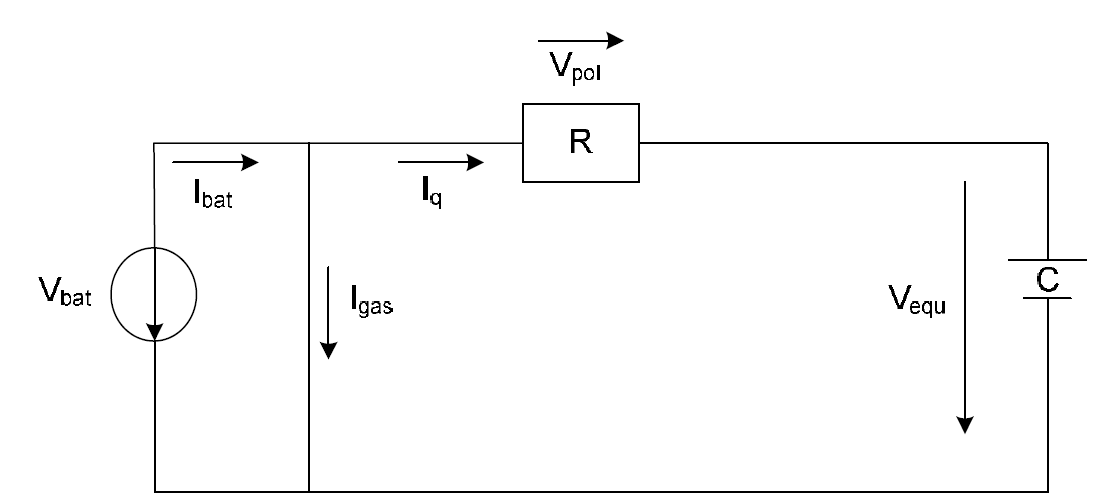
\includegraphics[scale=0.2]{EqivLeadAcid}\caption{Equivalent circuit for lead acid accumulator.}
\end{wrapfigure}%


The main variables for a common battery model are the voltage and
state of charge (SOC). Lets speak about a model of lead acid accumulator
from \cite{voutetakis2011design} - the model is generally valid for
batteries charged more than 20 \%, has relations for charging and
discharging and is parametrized by parameters that need to be computed
experimentally. (Needed to say, that there exist models even for overcharged
batteries and other specific cases.)

\[
I_{bat}=I_{q}-\frac{Q_{bat,nom}}{10}g_{0}\exp(\frac{V_{cell}}{g_{1}}-\frac{g_{2}}{T_{bat}})
\]
\nomenclature{$I_{bat}$}{battery current ($A$)}

The battery current is the reaction current ($I_{q}$) minus the gas
current losses, that are modelled using nominal capacity of accumulator
($Q_{bat,nom}$ in $Ah$), cell voltage, temperature and gassing current
parameters. The cell voltage is the equillibrium voltage plus polarization
voltage:

\[
V_{cell}=V_{equ,0}+\frac{V_{equ,l}SOC}{100}+V_{pol}
\]
\nomenclature{$V_{cell}$}{cell voltage ($V$)}

The equillibrium voltage is approximated linearily by its value at
$SOC=0$ and slope $V_{equ,l}$, the polarization voltage is different
for charging and discharging (with coefficients dependent on the battery):

\begin{align}
V_{pol,ch} & =U_{ch}a_{ch}(1-\exp(-\frac{I_{q,norm}}{b_{ch}})+c_{ch}I_{q,norm})\\
V_{pol,dch} & =U_{dch}(1-\exp(-\frac{I_{q,norm}}{b_{dch}})+c_{dch}I_{q,norm})(1+(g_{100}-1)\exp(\frac{SOC-100}{k_{100}}))
\end{align}
\nomenclature{$V_{pol,ch}$}{charging polarization voltage ($V$)}\nomenclature{$V_{pol,dch}$}{discharging polarization voltage ($V$)}

The indexes ``ch\textquotedbl{} stand for charging and ``dch\textquotedbl{}
for discharging. The parameters $g_{100},k_{100}$ are height and
slope parametes for fully charged battery ($SOC=100\%$).

A discrete model for a capacity of the battery is 
\[
Q_{bat,i}=Q_{bat,i-1}+I_{q}(t_{i}-t_{i-1})=Q_{bat,nom}SOC_{i-1}/100+I_{q}(t_{i}-t_{i-1})
\]
\nomenclature{$Q_{bat.i}$}{battery capacity ($J$)}

The state of charge of the accumulator is a fraction of the current
capacity at each time instant divided by its nominal capacity. So
for $SOC$ we have a model with efficiency ($\eta_{ac}$)\nomenclature{$\eta_{ac}$}{battery efficiency},
discharge rate ($\sigma_{ac}$)\nomenclature{$\sigma_{ac}$}{battery discharge rate}
and charge or discharge current $I_{ac}$\nomenclature{$I_{ac}$}{battery current (charge or discharge) ($A$)}.

\begin{equation}
SOC(t+1)=SOC(t)(1-\sigma_{ac})+I_{ac}\eta_{ac}(\Delta t)\label{eq:battmodel}
\end{equation}


$SOC$ cannot be directly measured, it needs to be derived from the
model or indirectly from experiements.\nomenclature{$SOC$}{battery state of charge}




\subsection{Electrolyzer and Fuel cell}

Electrolyzer and fuel cell both basically operate from a simple chemical
reaction (\cite{rayment2003introduction}) :

\[
H_{2}O\longleftrightarrow H_{2}+\frac{1}{2}O_{2}
\]


By adding (electric) power, the reaction occurs from left side to
the right, producing hydrogen and oxygen, whereas combining hydrogen
and oxygen allows us to get the energy back. The first way is the
basic function of electrolyzer and the latter is of the fuel cell.
By Faradays law, the (molar) quantity of produced/consumed hydrogen
is proportional to transfered charge.

Interesting details arise from the exact engeneering of both processes
(parameters like temperature, material of electrolyte or membrane,
catalyzators etc...), anyway the basic common variables are voltage,
current and temperature.

It is good to note, that hydrogen has the best heating value (energy
to fuel ratio). The higher heating value is $142.12\,MJ\,kg^{-1}$,
the pure standard heat formation of the product water. The lower heating
value is $120.21\,MJ\,kg^{-1}$, calculated from the fact, that the
product oxygen goes out unused as a steam (at said $150$ \textdegree C
). Electrolysis is not the only way to get hydrogen, other ways are
being considered too, for example by reforming natural gases.


\subsubsection{Electrolyzer}

Common types of electrolyzers are alkaline based (operates using an
alkaline solution) and proton exchange membrane electrolyzer (PEM
\nomenclature{PEM}{Proton exchange membrane}).

As presented in \cite{voutetakis2011design}, there are many ways
that lead to the voltage-current model of the electrolyzer: regression,
models based on analysis of processes on anothe, cathode and membrane
(and calculating then V-I relationship by subtracting from the open
circuit voltage the voltages of activation polarization and ohmic
polarization), and even rigorous CFD \nomenclature{CFD}{Computational fluid dynamics}
models.


\subsubsection{Butler Volmer equation}

In the work \cite{Stand-alonePowerSystems}, it is noted, that at
low voltages, the electrolyzer is more efficient, but generates small
amounts of hydrogen. The Butler-Volmer equation is used to model the
system:

\[
I=I_{0e}(\exp(\frac{(1-\alpha_{e})n_{e}F}{RT}(U-U_{eq}))-\exp(-\frac{\alpha_{e}n_{e}F}{RT}(U-U_{eq})))
\]


With unknown parameters $I_{0e}$, $\alpha_{e}$ (symmetry factor)
and $U_{eq}$. Hydrogen production rate is computed as follows: \nomenclature{$n_{H_2}$}{hydrogen production rate ($\frac{mol}{hr \cdot A}$)}

\[
n_{H_{2}}=\frac{N_{cell}I_{elec}}{n_{e}F}\eta_{F}
\]
\nomenclature{$N_{cell}$}{number of cells}\nomenclature{$I_{elec}$}{current through electrolyzer ($A$)}\nomenclature{$\eta_F$}{Faraday efficiency}

where $F$ is Faraday constant and $\eta_{F}$ is Faraday efficiency
(relation between theoretical and actual electron transfer, often
to be determined by experimental measure), $n_{e}=2$ \nomenclature{$n_e$}{Electrons in $H_2$}.



\paragraph{One empirical model}

\begin{equation}
V_{elec}=V_{rev,elec}+\frac{r_{1}+r_{2}T}{A_{elec}}I_{elec}+(s_{1}+s_{2}T+s_{3}T^{2})\log(\frac{t_{1}+t_{2}/T+t_{3}/T^{2}}{A_{elec}}I_{elec}+1)\label{eq:electr}
\end{equation}
\nomenclature{$V_{elec}$}{electrolyzer voltage ($V$)}\nomenclature{$A_{elec}$}{area of electrolyzer ($m^2$)}

This model primary expresses dependency on temperature (\cite{voutetakis2011design}).
There exists even empirical model for the faraday's efficiency, that
also accounts for the fact, that with decreasing current and/or higher
temperatures, the parasitic currents increase (because of the electrolyte).

\[
\eta_{F}=B_{1}+B_{2}\exp(\frac{B_{3}+B_{4}T_{el}+B_{5}T_{el}^{2}}{i})
\]
\nomenclature{$i$}{area current ($A/m^2$)}




\subsubsection{Fuel cell}

The exact process in fuel cell happens in this way:

\begin{eqnarray*}
H_{2} & \rightarrow & 2H^{+}+2e^{-}\\
\frac{1}{2}O_{2}+2e^{-} & \rightarrow & O^{2-}\\
2H^{+}+O^{2-} & \rightarrow & H_{2}O
\end{eqnarray*}


And the calculation (from \cite{olubukunmi2011solar}) for the amount
of hydrogen produced is:

\[
n_{H_{2}}=\epsilon\cdot0,01866\frac{mol}{hr\cdot A},\,m_{H_{2}}=\epsilon\cdot3,77\cdot10^{-5}\frac{kg}{hr\cdot A}
\]
\nomenclature{$m_{H_2}$}{hydrogen production rate (kilograms instead of mols) ($\frac{kg}{hr \cdot A}$)}...
where $\epsilon$ is the fuel cell efficiency:

The simplest way to model fuel cell V-I relationship is to look at
it as a reverse electrolyzer, this way is followed by the following
model from \cite{voutetakis2011design}.


\paragraph{First empiric model}

Takes into account the overvoltages (ohmic and activation), but not
effects of mass. The model computes the cell voltage $V_{fc}$\nomenclature{$V_{fc}$}{fuel cell voltage ($V$)}
using open circuit voltage $V_{o}$\nomenclature{$V_{o}$}{open circuit voltage for fuel cell ($V$)},
current density $i$ (in $A/m^{2}$), model parameter $b$, current
at the inflection point of the V-I curve $I_{d}$ and slope $\Delta$
at the linear stage of ohmic overvoltage:\nomenclature{$I_{d}$}{current at inflection point in fuelcell V-I curve ($A$)}

\[
V_{fc}=E+\frac{b}{\ln(1/I_{d}\,i)}-(\Delta-\frac{b}{4I_{d}})\,i
\]


The parameters ($K\in\{E,\,I_{d},\,b,\,\Delta\}$) \nomenclature{$K$}{general notation for one parameter in empiric model for fuelcells}
vary with fuel cell temperature $T$ and oxygen partial pressure $p_{O_{2}}$:\nomenclature{$p_{O_2}$}{oxygen partial pressue ($Pa$)}

\[
K=K_{1}+K_{2}T+K_{3}T\ln(p_{O_{2}})
\]


It is said, that this model is suitable more for low voltages and
powers. But it can be used even for electrolyzer ($p_{O_{2}}$ is
then the operating pressue for the electrolyzer at which the oxygen
is produced).


\paragraph{Second empiric model}

This model takes into effect even the mass transport limitation. For
computation of a cell voltage $V_{fc}$ and open circuit voltage $V_{o}$,
the following applies:

\begin{eqnarray}
V_{fc} & = & V_{o}-a_{T}\log(i)-ir+m\exp(il)\label{eq:usedfuelcell}\\
V_{o} & = & V_{rev,FC}+B\log(i_{o})\nonumber 
\end{eqnarray}


Where $V_{rev,FC}$ \nomenclature{$V_{rev,fc}$}{fuelcell, reversible voltage ($V$)}is
the reversible voltage, $i$ the current density (fuel cell current
per unit area of the electrode, in units of milliampers per square
centimeter),$i_{0}$ and $B$ the Tafel parameter ($i_{0}$ is the
value on the Tafel plot when the current begins to move away from
zero), $a_{T}$ the Tafel slope, $r$ the resistance (in $\Omega\cdot cm^{2}$),
and finally the model parameters $m$, $l$ representing the overvoltage
due to mass transport limits. All these parameters can depend on temperature.

Hydrogen and oxygen then flows according to this equations (by Faradays
law, already substitued $n_{e,H_{2}}=2,\,n_{e,O_{2}}=4$):

\[
H_{2,g}=\frac{N_{cell}I}{2F\eta_{F}}\,mol/s,\,O_{2,g}=\frac{N_{cell}I}{4F\eta_{F}}\,mol/s
\]


All these models are empirical and are important because of their
low computational complexity. For greater complexity, there are, of
course, more sophisticated models using partial differential equations.
For more in depth description, there is also a book about fuel cells,
that examines every aspect of fuel cell design and explains the details
of how fuel cells work \cite{larminie2003fuel}.

Lets add a word about the storage of hydrogen. The possibilities for
storage are to store it at the output pressue of the electrolyzer,
or at higher pressue or liquidified. These possibilities are covered
in most of presented resources and citations. If we wanted to store
the hydrogen in any other way, than at the output pressue, we would
need to add the compressor into the equation (like it is done in \cite{voutetakisdesign}).




\section*{\pagebreak{}}


\section{Optimization and optimal control - general theory}



Optimization is a rich field with many subproblems arising from the
specific problem settings. Optimal control is actually applied optimization
together with variational calculus \cite{milyutin1999calculus} and
has similar subproblems (or subclasses).

As (global) optimization is concerned about finding the minimum of
a function with number of parameters, optimal control theory takes
this idea to the next step and solves minimum of a functional (``objective
function'' or ``cost function\textquotedbl{} $J$ that consists
of final time objective and integrated Lagrangian) of a dynamic system,
evolving in time, controlled by a function (system dynamics).

\begin{align}
\mbox{minimize}\,J & =\phi(x(T),T)+\int_{0}^{T}L(x,u(x,t),t)\,dt\tag*{...cost function / objective function}\nonumber \\
\dot{x} & =f(x,u(x,t),t)\tag*{...system dynamics}\nonumber \\
x(0) & =x_{0}\label{eq:basiceqs}\\
g(x,u(x,t),t) & \leq0\tag*{...constraints}\nonumber 
\end{align}


In free final time case, the function $\phi$ is not present.

Problems from calculus of variations can be formulated as an optimal
control problem, so the ideas from this field apply in optimal control
too. Moreover, optimal control theory has methods for solving the
problem of controllability and observability and the presence of noise.

\stepcounter{subsection}


\subsubsection{Basic terms}

Optimization problems have many subclasses (\ref{fig:Optimization-Tree})
and optimal control is not an exception.\begin{wrapfigure}{o}{0.5\columnwidth}%
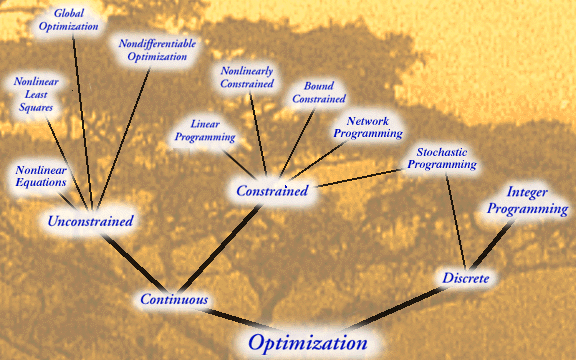
\includegraphics[width=0.5\textwidth]{treeoptimiz}\caption{\label{fig:Optimization-Tree}Optimization Tree, neos.mcs.anl.gov}
\end{wrapfigure}%




So, in formulating the problem, there are many decisions that need
to be made, or many features, that can be adressed. To get a grasp
of the field, lest summarize the most common features. (More details
can be found in the book \cite{bertsekas1995dynamic}, the developement
of this field over time is summarized in the article \cite{sargent2000optimal}).

First, the problem can be formulated in \textbf{finite time} or \textbf{infinite
time}, or the \textbf{time can be varied} too (``free time, fixed
endpoint'' problem vs ``fixed time free endpoint''). The model
can be\textbf{ continuous} or \textbf{discrete}, not only in \textbf{time,
but also in states}. Lastly, we can account for \textbf{statistical
uncertainities}. When we add probabilty to the problem, we will be
dealing with markov chains theory.

The goal, control policy, can be made \textbf{open loop} or \textbf{closed
loop} formulation. Closed loop does care for values and decisions
in intermediate states, whereas open loop control has the control
function predetermined in advance and does not rely on intermedate
states and values. Methods for solving optimal control problems are:
\textbf{dynamic programming}, \textbf{Hamilton Jacobi Bellman (HJB)
}\nomenclature{HJB}{Hamilton Jacobi Bellman (equations)}\textbf{
equations} and \textbf{Pontryagin maximum principle} (or minimum principle
... it is called by both names in literature). Only some of the problems
can be solved analytically, for example the class of \textbf{linear
quadratic control} problems, that can be solved through Riccati equations.

Long story short, there are two main approaches - direct methods and
indirect methods. Indirect methods take the optimal control problem
and reformulate it as differential equation problem with possible
boundary conditions - this approach is best used for continuous functions,
of course. Direct methods, on the other hand, would see the problem
as a problem of nonlinear programming

Both approaches are supported by the strength of calculus of variations
\cite{gelfand1964calculus} and both approaches are actually used
in numerical solutions.


\subsubsection{Hamiltonian of the system}

Many problem formulations could be efficiently written using Hamiltonian
of the system. We will use it too, so lets state the Hamiltonian as
a Lagrangian (from cost function) plus adjoint variable times system
dynamics, how the Hamiltonian is usually defined:

\begin{eqnarray}
H(x,u,\lambda,t) & = & L(x,u,t)+\lambda^{T}f(x,u,t)
\end{eqnarray}


Said efficiency comes from the fact, that the system dynamics is a
sort of a constraint and we translate constrained optimization problem
to unconstrained - the adjoint variable comes from this idea to introduce
lagrangian multipliers (as in \cite{EvansControlCourse,Lewis2012optimal,bryson1975applied})
or from HJB equations. There are two ways to get the equations presented
later, one gives the name ``adjoint variable\textquotedbl{} to one
of the derivatives, so it is conveniet to use the name. It is essential
for formulations, that will come later. Lets just note here, that
Hamiltonian is constant for systems with parametres independent on
time.

To summarize, the problem is then to optimize the value of Hamiltonian
- finding such optimal control function $u$, state function $x$
and costate function $\lambda$.\nomenclature{$u$}{usuall notation for control function}\nomenclature{$x$}{usuall notation for state}\nomenclature{$\lambda$}{usual notation for costate}


\subsubsection*{Dynamic programming}

Dynamic Programming is a principle well known for problems, that can
be decomposed into smaller subproblems. The principle is easy - if
the optimal solution of a problem can be composed from optimal solutions
of subproblems, we can use this information to build the solution.
Whenever this is true (needs, for example, additive cost function),
we just dont need to search the whole state space, but we can construct
the solution by constructing subsolutions one from another in a clever
order. Like, for example, the problem of finding the shortest path
in a graph.

Dynamic programming needs discretized problem formulation. Ultimately,
going to the limit with discretization points gives rise to the HJB
equations.


\subsubsection{Hamilton-Jakobi-Bellman equations}

HJB eqs. are partial differential equations of the problem (here we
need the Hamiltonian), the last equation is just system dynamic written
using Hamiltonian:

\begin{align}
J^{\star}(x(T),T) & =\phi(x(T),T)\\
-\frac{\partial J^{\star}}{\partial t} & =\min_{u}H(x,u,J_{x}^{\star},t)=L(x,u,t)+J_{x}^{\star}f(x,u,t)\nonumber \\
\dot{x} & =\frac{\partial H}{\partial\lambda}=f\tag*{...state equation}\nonumber 
\end{align}


When using this apporach, the first step to solve is to get the optimal
value function first and from that the other values.

Hamilton-Jakobi-Bellman equations from optimal control gave life to
the theory of viscosity solutions (more can be found in the articles
\cite{bardi2008optimal,dragoniintroduction,liu2013introduction}.)
These equations can be solved using finite element methods, but their
numerical stability is said to not be good in practise.


\subsubsection{Pontryagin principle of maximality, PMP}

The last step - or method - is principle of maximality (Pontryagin
principle of maximality, PMP \nomenclature{PMP}{Pontryagin maximum principle})
and can be - for continuous control functions - derived using the
HJB equations (as in \cite{bertsekas1995dynamic}). Using that, we
get to formulate equations for adjoint variable - the first equation
is pontryagin maximum principle and the second we get by differentiating
HJB equation, as in \cite{diehl2011numerical}. The last condition
is the transversality condition for fixed time free endpoint problem.



\begin{align}
u^{\star}(t,x,\lambda) & =\arg\min_{u}(H(x,u,\lambda,t))\phi(x(T),T)\\
-\dot{\lambda} & =\frac{\partial H}{\partial x}=\frac{\partial f^{T}}{\partial x}\lambda+\frac{\partial L}{\partial x}\\
\lambda(T) & =\nabla\phi(x(T),T)
\end{align}




As was said, we get the same results even from the perspective of
taking the system dynamic as constraint for lagrange multipliers.

In the presence of state constraints $x\in R=\{x\in\mathbb{R}^{n},\,g(x)\le0\}$,
PMP is formulated a bit differently \cite{EvansControlCourse} - we
need to define a function 
\begin{equation}
c(x,u)=\nabla g(x)\cdot f(x,u)
\end{equation}
 and the costate equation becomes: 
\begin{equation}
-\dot{\lambda}=\frac{\partial H}{\partial x}(x,u,t)+\mu\frac{\partial c}{\partial x}(x,u)
\end{equation}
While the PMP now states the existence of the function $\mu:\,[0,T]\rightarrow\mathbb{R}$.

Needed to say, that PMP equations are only necessary condition for
optimality, so analytical proof of existence and uniqueness is needed.


All these analytic methods will give us equations, to solve the equations
is a concern of numerical optimal control.


\section{Numerical optimal control}

Numerical optimal control can be, again, used to solve either continuous
or discretized problems. Heavily relies on the problem analysis and
follows the said methods. It would seem, that it is sufficient to
just solve HJB PDE's, but it is not used everytime. For example, the
problem is, so called, curse of dimensionality - when state and/or
control, has many components, the problem becomes exponentially hard
to solve. Suggested remedy, in the article \cite{diehl2011numerical},
is, for example, to approximate cost function by another means, for
example using neural network methods.  Second clue, to know when
to use state and costate equations, is, that when we want to have
continuous control function, we can just solve the boundary value
problem (as in, for example, \cite{wang2009solving}). When we want
to allow discontinuities, we need to rewrite the problem to nonlinear
optimization problem (an excellent book about this topic is \cite{chachuat2007nonlinear}).



\begin{figure}
\fbox{\begin{minipage}[t]{1\columnwidth}%
\begin{itemize}
\item HJB Equations - tabulation in state space
\item Indirect methods, Pontryagin - solve boundary value problem
\item Direct Methods - change to nonlinear programming

\begin{itemize}
\item Single shooting - discretized controls to NLP
\item Multiple shooting - controls and node start values discretized
\item Collocation - disretized controls and states\end{itemize}
\end{itemize}
%
\end{minipage}}

\caption{Numerical optimal control cases}
\end{figure}


As said above, the main classes are \textbf{indirect methods} (first
optimize then discretize) and \textbf{direct methods} (first discretize,
then optimize). Indirect methods result in algorithms similar to ODE
\nomenclature{ODE}{Ordinary differential equation} solvers, but the
resulting system can be badly conditioned or unstable in some cases.
Direct methods just rewrite the problem to the area of nonlinear programming
problem and then apply convenient solver.

There are three main cases of direct methods - \textbf{\textcolor{black}{single
shooting}}, \textbf{multiple shooting} and \textbf{collocation}.


\paragraph*{Single shooting}

discretizes the control to piecewise constant function and uses numerical
integrator for the evaluation of the cost function (ODE). This way
we get a finite dimensional optimization problem, which can be solved
by any nonlinear programming algorithm \cite{OptcontrNLP}, more in
section below.

Single shooting algorithm is usefull, but the stability can sometimes
depend heavily on starting value.


\paragraph*{Collocation}

discretizes both the control function and state function and approximates
the integral. We get larger system for nonlinear programming, but
the good news is that the system is sparse (in the meaning, that the
Jacobian has many zero elements). Collocation can treat better even
unstable systems, but refining the grid results in new problem with
higher dimensions.


\paragraph*{Multiple shooting}

discretizes the control, as single shooting, and additionally the
time scale. So it is called ``multiple'' shooting, because it works
like running single shooting algorithm repeatedly again from the starting
times $t_{i}$. Of course we need to add constraints for continuity
(the end values from the previous interval to be the same as the starting
values on the next interval). Multiple shooting algorithm results
in only a block sparse problem, but is easy to paralelize and can
treat even unstable systems well.

Numerous implementations of numerical optimal control are availible,
not only in MATLAB, but for example also in C++ in \cite{Houska2011a}.


\paragraph{Nonlinear programming (NLP)\nomenclature{NLP}{Nonlinear programming}}

Is an area of algorithms for optimizing nonlinear cost functions (on
constrained and unconstrained sets). Methods include derived algorithms
from ideas of gradient descend or newton method (applied on finding
a point where the gradient is zero), for example. Usually these methods
can also make use of derivatives (with said newton method on first
derivative we, for example, need also second derivatives) and that,
in case of optimal control and optimizing differential equations,
leads to the need of computing sensitivity equations. That means how
the functional depends on the choice of (discretized) control function
$\frac{\partial J}{\partial u_{i}}$. When not supplied, methods usually
compute these just by approximating. Algoritmical approaches for getting
the results for sensitivity are, for example External Numerical Differentiation,
Variational Differential Equations, Automatic Differentiation, Internal
Numerical Differentiation (that makes use of the equations written
directly in source code for numerical computation).

More details about computing sensitivity equations are for example
in \cite{Sensitivity20061553}. A suggested technique for solving
optimal control problems is, for example, Sequential quadratic programming,
SQP \nomenclature{SQP}{Sequential quadratic programming}, \cite{boggs1995sequential},
\cite{ottanumerical}. It is a method for solving nonlinear problems
with second derivatives; uses repeated subsolutions of quadratic programming
problems.

\pagebreak{}


\chapter*{Optimal problem algorithm for actual energy source configuration}

%\setcounter{chapter}{3}
%\setcounter{section}{0}
%\setcounter{subsection}{0}
%\setcounter{subsubsection}{0}
\stepcounter{chapter}
\addcontentsline{toc}{chapter}{Solution}

In this section we will apply the theory and methods to our setting
and problem (trying to focus on issues, that were not answered elsewhere).


\paragraph{Contribution of this work}

Now, lets emphasize, that other existing works tried to model the
problem using discontinuous functions and optimized only the system
parameters (for minimial cost) for given power managment strategy
or optimized only the power managment strategy (or decision constants
of the said strategy).

So our aim will be to optimize the global parameters against the cost
(using global optimization algorithms), but for each test case (values
of variables) to use the methods of optimal control theory to find
the best control strategy. That can be usefull in cases, where we
wonder about the following:
\begin{itemize}
\item How will the perception of the problem change for continuous formulation
of equations?
\item Will there be a case, when it is not valid to suppose, that for all
system parameters the optimal control strategy are still the same
through time?
\end{itemize}
At the end, we will discuss how can we use ideas from other works
or how to use the designed method in practical setting.

In the scope of this work, there will be developed an implementation
computing the values for an exact desired setting.




\section{Mathematical formulation}

This section will advance from writing the problem in terms of equations
to actually applying knowledge and methods for rewritting for numerical
solving


\subsection{Formulation of the optimal control strategy}

Since we are using continuous formulation of equations, we are able
to follow the optimal control theory for continuous cases (thats one
difference from other works).


\paragraph{Model using power}

We need to rewrite the setting using mathematical formulation - to
express the boundary conditions, the state variables $x(t)$, the
performance index $J()$, the control function $u(t)$ and the dynamics
of the system $\dot{x}=f(x,u,t)$ (using notation consistent with
the optimal control theory, see eqs. \ref{eq:basiceqs}). 

Lets express every state variable in energy, Joules, and control variables
in Watts, with exception for $u_{2}$\nomenclature{$u_2$}{current flow from hydrogen ($A$)},
that will be in ampers (see next).

Because we have two state variables - the state of charge of the accumulator
$B(t)$\nomenclature{$B(t)$}{energy stored in the accumulator ($J$)}
and the stored hydrogen $S(t)$\nomenclature{$S(t)$}{stored hydrogen ($2F \cdot mol$)}(in
the scripts the units are multiplied by Faradays constant times $n_{e}$
times number of moles - to not do conversion again for electrolyzer
and fuelcell), our state is two dimensional real valued function $x(t)=(x_{1}(t),x_{2}(t))=(B(t),S(t))$.
These quantities are bounded by $B(t)\leq B_{max}$\nomenclature{$B_{max}$}{maximal energy in battery ($J$)}
and $S(t)\leq S_{max}$\nomenclature{$S_{max}$}{maximum of hydrogen in tank ($2F \cdot mol$)},
bounds to maximal battery charge and maximal hydrogen stored (in means
of power we used to create the hydrogen). 

The boundary condition is the source power from solar collectors and
power demand, defined as $P_{src}(t)=P_{in}(t)-P_{demand}(t)$\nomenclature{$P_{src}$}{source power as energy from solar collectors minus electricity demand ($W$)},
difference between input power and power demand (in Watts). Usually
the data would look like in figure \ref{fig:First-seven-days}.
\begin{figure}
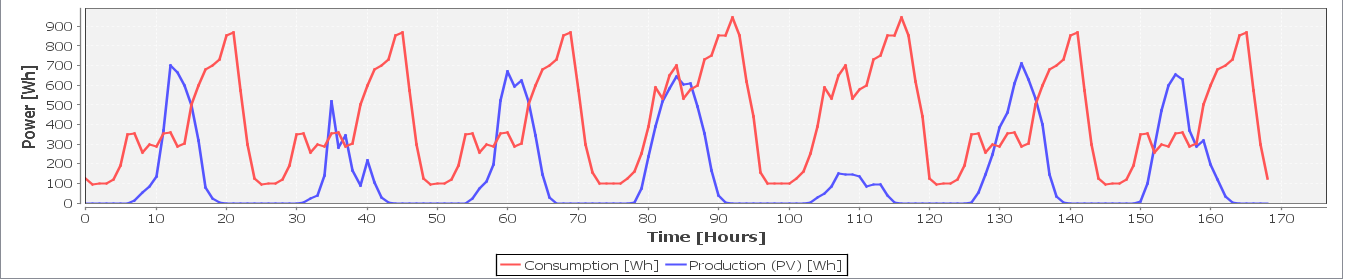
\includegraphics[width=1\textwidth]{oneweekofdata}\caption{\label{fig:First-seven-days}First seven days of availible data (power
production from PV panels from UJV �e�). As the data start with wednsday,
notice bigger consumption over weekends (in the middle).}


\end{figure}
The control function $u$ is also a two dimensional function of time
and will define the power flow:
\begin{itemize}
\item the first component tells us about charging/discharging the battery:


\[
\dot{(B)}(t)=P_{batt}(u_{1})-\sigma B(t)
\]



Using this equation we can model the efficiency by setting $P_{batt}(u_{1})=u_{1}\eta_{batt}$
and also the result of auto discharge $\sigma$.
\begin{itemize}
\item $u_{1}>0$ ... We are charging the battery, using the power $u_{1}$.
There is a bound, how much power can we give to the battery $u_{1}\in[P_{batt+min},P_{batt+max}]$\nomenclature{$P_{batt+max},P_{batt+max},$}{Maximal/minimal power flow to the battery ($W$)}
\item $u_{1}=0$ ... Battery disconnected
\item $u_{1}<0$ ... We are discharging the battery, getting the power $-u_{1}$.
There is a bound, how much power we can get from battery $-u_{1}\in[P_{batt-min},P_{batt-max}]$\nomenclature{$P_{batt-max},P_{batt-max},$}{Maximal/minimal power flow from the battery ($W$)}
\end{itemize}
\item The second component tells us about the current flowing from the hydrogen
source:


\[
\dot{(S)}(t)=P_{H_{2}}(u_{2})
\]



Definitely the term will be different for $u_{2}$ positive and negative,
because this equation models two different devices:
\begin{itemize}
\item $u_{2}>0$ ... The electrolyzer is turned on, using the power$P_{H_{2}}(u_{2})$.
There is a bound, how much current can flow $u_{2}\in[P_{H_{2}+min},P_{H_{2}+max}]$\nomenclature{$P_{H_{2}+min},P_{H_{2}+max}$}{Maximal/minimal current to electrolyzer ($A$)}
\item $u_{2}=0$ ... No change in hydrogen supply
\item $u_{2}<0$ ... The fuel cell is turned on, giving us the power $P_{H_{2}}(u_{2})$.
There is a bound, how much current we can get $-u_{2}\in[P_{H_{2}-min},P_{H_{2}-max}]$\nomenclature{$P_{H_{2}-min},P_{H_{2}-max}$}{Maximal/minimal current from fuelcell ($A$)}
\end{itemize}

Again, here we can model the efficiency (for example $P_{H_{2}}(u_{2})=\frac{N_{cell}u_{2}}{2F\eta_{F}}\eta_{H_{2}}$
for $u_{2}<0$ - the current would flow to the fuelcell, so we use
the equation for fuelcell \ref{eq:usedfuelcell} multiplied by efficiency)
and even nonlinear characteristics of the efficiency. This design
follows the wise rule, that the electrolyzer and fuel cell should
not operate simultaneously (because that would be a waste of power).
The bounds are, for example, the technical specifications set by the
manufacturer. Why do we use current for $u_{2}$ as a variable and
not power? Because the model equations \ref{eq:usedfuelcell} give
us how the voltage depends on current (and from that we can get the
power dependency on current and thats the function $P_{H_{2}}(u_{2})$).

\end{itemize}
Also in many cases in literature, the result of the analysis of the
optimal control problem is, that the actual control function is so
called bang-bang control or bang-off-bang control. These controls
are called this way, because they only use maximal allowed values
and zero (turned off). In our case it would not be wise to follow
this path, because the efficiency, in the means of power, varies.



So, once again and nicely written, the dynamics of our system is:
\begin{eqnarray}
\dot{x} & = & f(x,u,t)\\
\dot{\left[\begin{array}{c}
B(t)\\
S(t)
\end{array}\right]} & = & \left[\begin{array}{c}
P_{batt}(u_{1})\\
P_{H_{2}}(u_{2})
\end{array}\right]+\left[\begin{array}{c}
-\sigma\cdot B(t)\\
0
\end{array}\right]\nonumber 
\end{eqnarray}
To finish our formulation, we want to find the minimizing control
function $u^{\star}$ (and the corresponding minimizing trajectory
$x^{\star}$ and costate $\lambda^{\star}$ - will be introduced later)
to minimize the performance index

\begin{eqnarray}
J & = & \phi(x(T),T)+\int_{0}^{T}L(x,u,t)\,dt\nonumber \\
 & = & hcost(S(T))+bcost(B(T))+\int_{0}^{T}pcost(P_{src}-P_{batt}-P_{H_{2}})\,dt\label{eq:hcostbcostdef}
\end{eqnarray}
where $hcost(x)$ is a function that gives a price for hydrogen,
$bcost(x)$, price for power in the battery and $pcost(x)$ is a function
that translates power exchange with the grid to its money cost. Generally
$pcost(0)=0,\,pcost(x)\cdot x\geq0,\,|pcost(x)|\leq|pcost(-x)|$ and
all the functions are bounded on bounded intervals.

That simply says, that for not using the grid we pay nothing, selling
gives us money, by buying we lose money and that selling the power
to grid would not give us such an amount of money as we would lose
by buying the power.

Generally we can think of any $pcost$ function, in the solution and
scripts below we will simply use $pcost(x)=c_{1}x\mbox{ if }x\geq0\mbox{, otherwise }=c_{2}x$,
for $c_{1},c_{2}\geq0$.

As we will see later, the most important thing is, that the function
$J[x(u)]$ would be continuous.


\subparagraph{Note}

If we wanted to not optimize the cost, but the effectivity (in means
of power), we would simply use $L(x,u,t)=|P_{src}-P_{batt}-P_{H_{2}}|,\,\phi=0$.

Thats exactly the power, we are outputting to the net (or withdrawing
from) over selected time interval $[0,T]$. We are not interested
in the final value (even not in minimizing any function of the final
state) so it is classified as final state free problem.


\paragraph{Models for business problems}

As a note, every optimal control problem, whose aim is to find the
optimal strategy and the minimum of the functional, can be upgraded
so it can compute parameters for the most economic installation. The
adjustment is just adding parameters to the equation, that will allow
us to use components with different efficiency and tie these to a
cost. The cost, in turn, can then be added to the cost functional
(with keeping an eye on the fact that then the physical units will
become a currency and making any necessary adjustments) and the parameters
can be also passed to the numerical optimalizator.

For the test run in the scripts attached, very simple models are used,
that bind the efficiency quadraticaly to cost (bounded on an interval).




\subsection{Construction of solutions and rewriting the problem}

Now we will look at different formulations and used methods from the
literature, that will give us necessary conditions for minimality,
even from different views.


\paragraph{Hamiltonian}

The Hamiltonian of our system, using $\lambda\in\mathbb{R}^{2}$ as
lagrange multipliers is 
\begin{eqnarray}
H(x,u,\lambda,t) & = & L(x,u,t)+\lambda^{T}f(x,u,t)\\
 & = & |P_{src}-P_{batt}-P_{H_{2}}|+\lambda_{1}(P_{batt}(u_{1})-\sigma\cdot B(t))+\lambda_{2}P_{H_{2}}(u_{2})\nonumber 
\end{eqnarray}


By the way, because our state equations do not depend on time, our
Hamiltonian is constant. If we would include the fact that, for example,
the battery gets old and less efficient in time, the hamiltonian will
suddenly become non constant.



Additionally, in the presence of state constraints (for example $x\in[0,B_{max}]\times[0,S_{max}]\iff\{x\in\mathbb{R}^{2},\,g(x)\le0,\,g(x)=-((x_{1}-\nicefrac{1}{2}B_{max})^{2}+\nicefrac{1}{4}B_{max}^{2})((x_{2}-\nicefrac{1}{2}S_{max})^{2}+\nicefrac{1}{4}S_{max}^{2})\}$),
the definition of Hamiltonian alone is not sufficient and the theory
usually also defines the function 
\begin{equation}
c(x,u)=\nabla g(x)\cdot f(x,u)\label{eq:defc}
\end{equation}
 (that will be used later).


\paragraph{Conditions for minimum}

Other (necessary) conditions for minimum are: (state equation, costate
equation, boundary conditions)

\begin{flalign}
\dot{x} & =\frac{\partial H}{\partial\lambda}=f\tag*{...state equation}\nonumber \\
-\dot{\lambda} & =\frac{\partial H}{\partial x}=\frac{\partial f^{\mathsf{T}}}{\partial x}\lambda+\frac{\partial L}{\partial x}\tag*{...costate equation}\nonumber \\
x(t_{0}) & =(0,0)\tag*{...boundary condition}\nonumber \\
0 & =(\phi_{x}+\psi_{x}^{\mathsf{T}}\nu-\lambda)^{\mathsf{T}}|_{T}dx+(\phi_{t}+\psi_{t}^{\mathsf{T}}\nu+H)^{\mathsf{T}}|_{T}dT\tag*{...boundary condition prototype}\nonumber \\
0 & =\psi(x(T),T)\tag*{...final state constraint (if present)}\\
0 & =\lambda^{\mathsf{T}}|_{T}dx+H^{\mathsf{T}}|_{T}dT\tag*{...boundary condition in our case \ensuremath{(dT=0)}}\nonumber \\
\lambda_{i}(T) & =\frac{\partial\phi}{\partial x_{i}}(x(T),T)\tag*{...boundary condition for costate (for free final state)}\nonumber \\
\lambda_{i}(T) & =0\tag*{...boundary condition for costate in our case}\nonumber \\
\end{flalign}





\paragraph{Pontryagin minimum principle}

Because values of control function are bounded (maybe even discrete
for degenerated intervals), we need to use Pontryagin maximum principle
(we are dealing with constrained input problem) �the Hamiltonian must
be minimized over all admissible $u$ for optimal values of the state
and costate.'' If we had continuous control function, the problem
could be tackled by more traditional approach using derivative of
Hamiltonian with respect to $u$.

In other words $H(x^{\star},u^{\star},\lambda^{\star},t)\geq H(x^{\star},u,\lambda^{\star},t)$
for all admissible $u$. (We have this instead of the stationary condition
$0=\frac{\partial H}{\partial u}=\frac{\partial L}{\partial u}+\frac{\partial f^{T}}{\partial u}\lambda$)

In the presence of state constraints (``maximum principle for state
constraints\textquotedbl{}), we have the existency of a costate function
$p^{\star}$ and a function $\lambda^{\star}$, such that: 
\begin{eqnarray}
\dot{p}^{\star}(t) & = & -\nabla_{x}H(x^{\star}(t),p^{\star}(t),u^{\star}(t))+\lambda^{\star}(t)\nabla_{x}c(x^{\star}(t),u^{\star}(t))\\
H(x^{\star},p^{\star},u^{\star}) & = & \max_{u}\{H(x^{\star},p^{\star},u)\,|\,c(x^{\star},u)=0\}
\end{eqnarray}


... for $u^{\star},\,x^{\star}$ solving the control problem ( eqs.
\ref{eq:basiceqs} ) and function $c$ defined above \ref{eq:defc}.
(Instead of simple $-\dot{\lambda}=\frac{\partial H}{\partial x}=\frac{\partial f^{T}}{\partial x}\lambda+\frac{\partial L}{\partial x}\mbox{ ...costate equation}$.)


\paragraph{Hamilton Jacobi Bellman}



The equation for developement of the optimal cost (computed backwards)
is 
\begin{eqnarray}
J^{\star}(x(T),T) & = & \phi(x(T),T)\\
-\frac{\partial J^{\star}}{\partial t} & = & \min_{u}H(x,u,J_{x}^{\star},t)=L(x,u,t)+J_{x}^{\star}f(x,u,t)\nonumber 
\end{eqnarray}


And to get $u^{\star}$ using HJB and Minimum principle:

\begin{eqnarray}
u^{\star}(t,x,\lambda) & = & \arg\min_{u}(H(x,u,\lambda,t))\phi(x(T),T)
\end{eqnarray}



\subsection{Approach using direct methods}

Above methods and conditions for minimum come from the indirect approach.
Allowing countable number of discontinuities would rise the need to
rewrite the problem, as in \cite{gelfand1964calculus}. If we would
like to use direct methods with functions with discontinuities, the
thoughts will go in different way (eg. not using the notation of Hamiltonian).


\subsubsection{Ritz method, finite differences and existence}

As an important known result about direct methods, the direct way
to get to the minimum is the following (using \cite{gelfand1964calculus}
as a reference, where also proofs can be found):

In a general situation (application to our specific case will come
later), where we want to evaluate a functional $J[y]$ depending on
a function $y$ from an general function space $\mathcal{M}$ ($y\in\mathcal{M}$),
we first construct an approximating sequence of spaces $\mathcal{M}_{i}$.
Each space $\mathcal{M}_{i}$ is defined by the basis functions $\{\varphi_{i}\}_{i=1}^{n}$,
such that their every linear combination $\sum^{n}\alpha_{i}\varphi_{i}$
together make the whole particular space $\mathcal{M}_{i}$. The sequence
of spaces will need to approximate (in subset sense $\mathcal{M}_{1}\subseteq...\subseteq\mathcal{M}_{i}\subseteq...\subseteq\mathcal{M}$)
the space $\mathcal{M}$ in which we would like the solution to lie.
This approach is called Ritz method.

Note, that the space $\mathcal{M}$ is likely to be infinite dimensional,
because the solution is, of course, a control function.


\paragraph*{Definition of complete sequence}

Approximating sequence of spaces is called complete, if, for any given
$y\in\mathcal{M}$ and $\epsilon>0$, we can have a function $y_{n}$
(of the form of linear combination) that differs less than epsilon
from the given function - $\left\Vert y_{n}-y\right\Vert <\epsilon$.\medskip{}


The convergence results then continue in this way:


\paragraph*{Theorem}

If a functional $J[y]$, $y\in\mathcal{M}$ is continuous (in the
norm of the space $\mathcal{M}$) and if a sequence $\mathcal{M}_{i}$
is complete, then $\lim_{n\rightarrow\infty}\mu_{n}=\inf_{y}J[y]$
($\mu_{n}$'s are realized by functions $y_{n}\in\mathcal{M}_{n}$,
that is then, in fact, a minimizing sequence of functions for the
functional $J[y]$).\medskip{}


The finite differences idea then adds, that the approximation in each
particular space is done by piecewise linear function.

Together then, if we have a sequence ($y_{n}$), of optimal solutions
of our problem constrained to space $\mathcal{M}_{n}$, we are approaching
the limit if the given functional is continuous.


\subsubsection{The application of Ritz method}

Does our problem, from the point of view of direct methods from calculus
of variations, have this property?

The space $\mathcal{M}$ is, in our case, defined as the space of
real valued functions $y(t)=(x(t),u(t)):\,\mathbb{R}^{4}\rightarrow\mathbb{R}$,
that are bounded on a bounded interval, $x(t)$ is continuous, and
do satisfy the state equation $\dot{x}=f(x,u,t)$ and $J$ is the
cost function of our problem, that was given by (in \ref{eq:hcostbcostdef}):

\begin{eqnarray*}
J[x,u] & = & \phi(x(T),T)+\int_{0}^{T}L(x,u,t)\,dt\\
 & = & hcost(S(u(T),x(T)))+bcost(B(u(T),x(T)))+\\
 &  & +\int_{0}^{T}pcost(P_{src}(x(t))-P_{batt}(u(t),x(t))-P_{H_{2}}(u(t),x(t)))\,dt
\end{eqnarray*}


And because everything comes down to functions $P_{batt}$ and $P_{H_{2}}$...
\begin{eqnarray}
\dot{\left[\begin{array}{c}
B(t)\\
S(t)
\end{array}\right]} & = & \left[\begin{array}{c}
P_{batt}(u_{1})\\
P_{H_{2}}(u_{2})
\end{array}\right]+\left[\begin{array}{c}
-\sigma\cdot B(t)\\
0
\end{array}\right]
\end{eqnarray}
... that are selected to be continuous (see models presented before
- \ref{eq:usedfuelcell}, \ref{eq:electr}, \ref{eq:battmodel} -
it is not only physically-wise selection that makes approximating
easier, computation faster, but it also gives us the needed results
here), we just need to clarify our demands on functions $hcost$,
$bcost$ and $pcost$ - to be continuous. Because these functions
just translate amouts of physical variable to cost in money, we can
assume continuity without causing any harm. 

In this analysis we ommited any constraints, but given the fact that
the constraints are, in the basic sense, constant, not dependent on
anything (because they just limit the maximal allowed powers of components),
they are not going to affect continuity in the presence of multipliers,
or any clever tricks meant to incorporate the multipliers (and they
also dont affect the existence of minima, because they constrain the
spaces on which we are searching for the minima).

Our functional is, in the end, easier to work with, than normally
presented problems from the calculus of variations, because we do
not have derivatives of the control function in our functional.





\begin{comment}
otazky

$\dot{x}=f(x,u,t):\dot{\left[\begin{array}{c}
SOC(t)\\
S(t)
\end{array}\right]}=\left[\begin{array}{c}
P_{batt}(u_{1})\\
P_{H_{2}}(u_{2})
\end{array}\right]+\left[\begin{array}{c}
-\sigma\cdot SOC(t)\\
0
\end{array}\right]$ minimize the performance index $J=\int_{0}^{T}|P_{src}-P_{batt}-P_{H_{2}}|\,dt$

poznamky z konzultace s Kurzikem 14082014

nejdriv jestli to existuje jestli mi ty omezeni na rozsah nezkazi
existenci - to je potreba overit

v roubickove knize 260, relaxace proto abych to mohl resit

rizeni je z kompaktni mnoziny

box constraints minimalizuju funkci a 

gradientni metody jsou supr pro konvexni ulohu - tam vlastne vim ze
sem v minimu. Muze bejt lepsi druha mocnina kviuli kvadraticky strukture.
ta absolutni hodnota

v numerice to nebude hladky takze na gradient by byl problem, tam
by byla absolutni hodnota - takze lepsi kvadratickej, to muzu zkusit.

fortran - optimization tree mittleman - plato asu

----------->-Numericky kody brat z http://plato.la.asu.edu/bench.html<\textcompwordmark{}<---------------------------

---------------

OTAZKA - Jak vyjadrim, ze u (ridici funkce) a x (stavova promenna)
je omezene (nejakym uzavrenym intervalem)? Jak se to projevi na rovnicich?

OTAZKA - Jak postupovat dal? Jaky numericky resic (c++ idealne) se
da pouzit? Je jich hrozna hromada:

Hodi se dal posutpovat spis Hamilton jakobi bellmanem, dynamickym
programovanim s diskretizaci, nebo principem maxima? Co je nejlepsi
z hlediska programovyho/numerickyho nejrychlejsiho? Co se pouziva?

OTAZKY ohledne PDR a viskoznich reseni:

-OTAZKA jak resit pomoci HJB a vizkoznich reseni? Staci MKP? Jak na
to?

-OTAZKA - jsou viskozni reseni zobecneny slabyma resenima z nami zname
PDR 1?

otazka - Co znamenaji posledni podminky v optimal control strany 123

others

OTAZKA - jde nas problem vyresit jako linear quadratic regulator?
To pak ma analyzticky reseni! a nemusim diskretizovat.

protiOTAZKA - co by se zmenilo, kdybych tam dal absolutni hodnotu
misto kvadratu? otazka co by se zmenilo kdybych tam nemel kvadrat,
ale absolutni hodnotu v hodnotici funkci?

...
\end{comment}







\section{Applied numerical procedures and results}

Using all previously mentioned, we developed a program capable of
answering the following questions:
\begin{itemize}
\item ``What is the most economic setting for photovoltaic and hydrogen
system and what is the specific power managment strategy (the optimal
control function) of such system?\textquotedbl{}.
\item ``What is the most economic control function for a specified time
scale, given a prediction of consumption and energy generation\textquotedbl{}
\end{itemize}
From now on, we will look on the second, easier question, with the
goal to verify the effectivity of numerous NLP solvers. So, lets suppose,
that we already have measured yearly power consumption and have already
installed photovoltaic panels and measured power output. If it is
not this case, we can, of course, use the model and approach from
\cite{Stand-alonePowerSystems} to get the estimated power output
from manufacturers datasheets. If we would like to answer the first
question, the only remaining work would be to add the equation tying
together the cost of a PV panels and other equipment and their effectivity.

Lets now have a look at all the implementation details and all the
used tools (because this way it would make the actual usage of the
scripts less time consuming work) and the accompanynig numerical experiments.


\subsection{Setting up the constants}

Two datasets standing for the boundary conditions of power consumption
and demand are supplied. The first data of generated solar energy
and house consumption were taken from this dataset \url{http://www.networkrevolution.co.uk/project-library/dataset-tc5-enhanced-profiling-solar-photovoltaic-pv-users/}
(using the monthly average averaged with weekday average for weekdays
and monthly average averaged with weekends average for weekends) and
through the scripts, the results are in a file \texttt{data.txt}.
The second dataset is a dataset that was also used in planning of
a real standalone system in the work \cite{VyrobaAVyuziti}, \texttt{data2.txt}.
(The first dataset was used in first experiments, in this text there
will be presented the data from the second dataset to allow comparsion.)

For setting the constants for electrolyzer and fuelcell empiric models,
we used the dataset \cite{Bauer:www.h2fc-fair.com} and a plot digitizer
software from \url{http://plotdigitizer.sourceforge.net/}. The model
parameters were fitted using MATLAB fitting toolbox (and from the
results below we can see, that the empiric models are indeed usefull
and sufficient). The source codes are in the directory ``fit\textquotedbl{}.

\begin{figure}
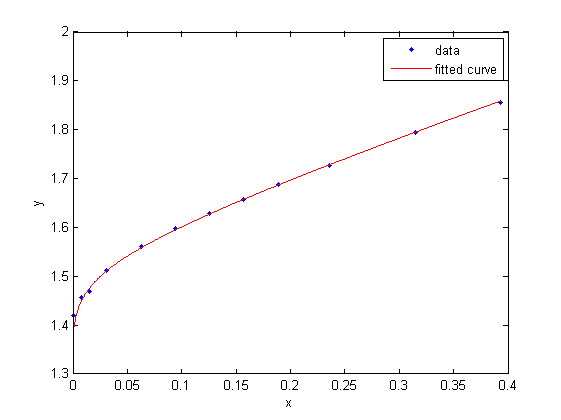
\includegraphics[width=0.45\textwidth]{fittedelectrolyzerplot}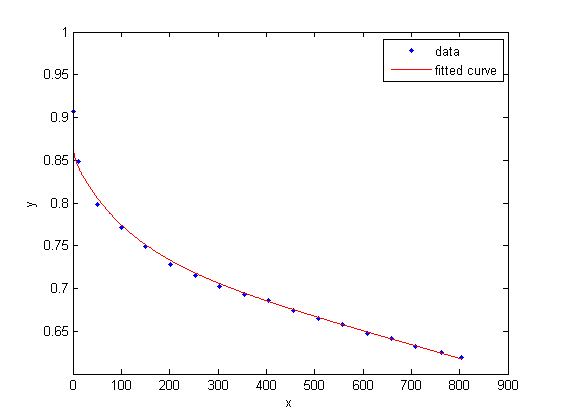
\includegraphics[width=0.45\textwidth]{fittedfuelcell}

\caption{Results of the fitting for electrolyzer (left) and fuelcell (right),
x axis is current density ($mA\cdot m^{-2}$ ), y axis is voltage
($V$). Actual values of parameters are kept in the file \texttt{consts.m}
together with all the other model constants and numerical settings.}
\end{figure}



\subsection{The scripts and usage}

First attempt was to use the ACADO optimization toolkit. Even though
the scripts (and tests) were not able to run completely, the source
codes using this library are also attached, in the directory AcadoLinearVersion
(waiting for the next release of the toolkit).

The next step was to use MATLAB and to write multiple shooting algorithm
(as was said, in a way to reformulate the optimal control problem
as NLP problem), the formulation is independent on actual solver used
and so it is able to run with MATLABs original fmincon function and
with any algorithm from OPTI toolbox (\url{http://www.i2c2.aut.ac.nz/Wiki/OPTI/}).
In the case of algorithm breakdown on a specific problem setting,
we can just easily switch to a different algorithm.

All used approaches to the problem are reported with respective sources
in these directories:
\begin{itemize}
\item Directory \texttt{MatlabSinglShooting1} contains implementation using
single shooting technique. This implementation was not effective for
this problem.
\item In the main directory, there is an implementation of multiple shooting
using MATLAB function fmincon.
\item Directory \texttt{TrySensitivity} contains the same problem implementation
with multiple shooting, but with employed sensitivity equations for
computing the derivatives. This approach has not proved to be working
effectively (probably because the precise computation of the derivatives
results in breakdown of the algorithm more often, than it did when
approximating them).
\item Directory \texttt{4dformulation} contains the code of a slightly differently
formulated problem, with 4 control functions (one for electrolyzer,
one for battery input, one for battery output and one for fuelcell)
in an attempt to try to cure said problem with derivatives, using
more dimensional problem, with only positive valued control functions
and more constraints. Unfortunately this approach failed, because
the resulting matrices in the computation were detected to be badly
conditioned by the algorithms.
\item Directory \texttt{Opti} contains the code for multiple shooting using
Opti toolbox solver.
\item Directory \texttt{AsBusiness} has sample scripts for optimization
of the cost - variables that influence the efficiency of the fuelcell
are added to the formulation, optimizer and final cost.
\item Directory \texttt{Test} contains all the code for the numerical test
cases presented below.
\end{itemize}
All the matlab scripts in each directory follow this structure:
\begin{itemize}
\item \texttt{main.m} - main file, executing in matlab will execute the
whole computation
\item \texttt{ctr.m} - function for computing the constraints (physical
and the ones resulting from multiple shooting approach)
\item \texttt{obj.m} - computing the objective function for optimization
\item \texttt{fun.m} - computing the whole equation, integration over the
time
\item \texttt{state.m} - evaluation of state equation
\item \texttt{statesens.m} - script for computing sensitivity equations
\item \texttt{consts.m} - file for storing the constants and options defining
the problem
\item \texttt{dispopt.m} - script for displaying graphs
\item \texttt{nlpoutfun.m} - script for displaying the approximations after
each iteration
\item \texttt{interpt1qr.m} - script for fast linear interpolation of the
source data
\item \texttt{controldata} - points on piecewise lienar function defining
the power demands
\item \texttt{dispsaved.m} - the script that would print the graphs like
in this work and compute the constraint violation and final cost.
\end{itemize}
Every variation of the scripts can be run in the same manner - executing
\texttt{main.m}. The solved problem is set to examine the effectivity
over one year period (or one week in the main folder). You can also
notice rescaling constants in \texttt{consts.m} - because letting
the integrators integrate functions depending on very high time ranges
in basic physical units (seconds) would take unreasonable amount of
time (also because the boundary conditions are set to change on hour
by hour basis and that means that nothing interesting happens for
the numerical integrator that tries to watch for sudden changes and
keep the precision).

For more discretization points the program becomes, of course, slower.
If we want to see some results earlier, we can set the constants ``Data.cLogBegin''
and ``Data.cLogEnd'' in \texttt{consts.m} to specify at which power
of two discretization points to begin and at which to end. This also
affects the selection of the initial values - on the first run they
are set randomly and on each consecutive run they are copied from
previous run (this is because the selection of initial point in the
search space can affect the outcome of certain optimalizators and
also their running time).

\begin{comment}
The program can operate in different modes:
\begin{enumerate}
\item global and control optimization - searches for the best setting against
costs using optimal control specific for each test case (i.e. runs
case 3. as a subroutine).
\item global optimization using PMS - searches for the best setting against
costs using only defined power managment strategies.
\item Simulation using optimal control - given the data, uses optimal control
algorithm to find optimal control for this one case
\item Simulation using PMS - given the data and PMS, simulates the system
\end{enumerate}
Source codes and program executables are attached in the electronic
version.
\end{comment}





\subsection{The numerical experiments}

The scripts will start solving the problem on discretized control
function to number of discretization points beginning at $2^{\mbox{cLogBeg}}$
and ending at $2^{\mbox{cLogEnd}}$ (constants from \texttt{consts.m}),
using the results from previous run as a starting point for the next
run. Some iterations can fail to satisfy the bounds, thinking that
the problem is infeasible, because at a lower number of discretization
points, achieving the result might be difficult or impossible. This
flaw is fortunately automatically fixed when the number of discretization
points grows bigger, because higher number of availible decision points
can steer the system to allowed set of states.

For correct one-year long prediction, the optimization process would
take long time ($2^{14}$ discretization points would require more
than 4 days of processor time per iteration), so we would chose smaller
time scale for testing purposes - one day and $2^{5}$ discretization
points. The main goal is to explore, which NLP solvers would perform
reasonably well on this type of problem. 

This test case was set up to control a production of one day, where
the photovoltaic power income was less than it would be needed and
the test case starts with empty batteries and fuel tank. The goal
is to observe lesser cost of electricity over the day.

The currency is set to a virtual one, where to buy an unit of power
costs 200 units, to sell it costs 100 units and the energy remaining
in batteries and fuel at the end of the run can be sold for 150 units.
The efficiency of the battery is set to 70\% and the fuelcell is considered
ideal in this test case (to see if the algorithm would use the fuelcell
even though it's nonlinear characteristic).

The initial point is chosen to be random, because some solvers would
consider zero to be a local optimum.


\subsubsection{Understanding the results}

After each iteration, the environment will show the state of the optimization
in 4 graphs, like in \prettyref{fig:Filtersd}.

Left top graph shows the state of energy in battery and hydrogen in
tank, right top graph shows the evolution of the cost function in
time (this curve is an integral of our virtual currency flow, which
is just weighted power flow to the system), left bottom graph shows
the control function (2 dimension - power to battery and current to
hydrogen - so two lines) and right bottom graph shows the state trajectory.
The axes in each subfigure are scaled for better run of the algorithm.

At the beginning, the algorithm starts from a point far from optimum.
As for multiple shooting, the graph for states is not even continuous
during the computation, because the solvers need more iterations to
guess correctly the beginnings of the states.


\subsubsection{Results of test runs}

Usually, the results verify, that with lower number of discretization
points, the algorithms tend to fail, because they are not able to
even meet the provided conditions on such small scale level - the
power input and demand oscillates faster, than the number of control
points allows for compensation.

From MATLAB and OPTI toolbox, we have applied the algorithms listed
in the table \ref{fig:Results-of-test}, together with the evaluation
of the success of every solver. 

\begin{figure}[H]
\begin{centering}
\begin{tabular}{|c|c|c|c|}
\hline 
algorithm (ndisc=32) &  & optcost & max constraint violation\tabularnewline
\hline 
\hline 
SQP &  & -2.072860e+08 & 2.851336e-05\tabularnewline
\hline 
active-set & spustit &  & \tabularnewline
\hline 
interior-point & bezi &  & \tabularnewline
\hline 
IPOPT & spustit &  & \tabularnewline
\hline 
NLOPT & \ref{fig:NLOPT} & -1.062047e+09 & 7.919988e+06\tabularnewline
\hline 
filtersd & \ref{fig:Filtersd} & -2.429403e+08 & 7.920000e+06\tabularnewline
\hline 
lbfgsb &  &  & \tabularnewline
\hline 
PSWARM & nesel &  & \tabularnewline
\hline 
\end{tabular}
\par\end{centering}

\caption{\label{fig:Results-of-test}Results of test runs.}
\end{figure}




All the solvers managed to find a better strategy than to just buy
the power from the grid (which can be seen from the top right graph
that would go steeply linearly down), unfortunately some of them did
'cheat' in a sense, that the constraints were not satisfied. The best
performance can be observed for SQP (Sequential quadratic programming),
which is in line with the suggested approach from various sources.

The solver converged to make decisions (as seen in figure \ref{fig:SQP})
copying the peaks from boundary conditions and mostly using the ideal
fuelcell over the battery - even in spite of accompanying nonlinearities
- and used the battery as a backup for one moment of need. In reality,
the roles would be reversed and fuelcell used more as long term storage,
but that might not be the same challenge for the numerical test of
the solver.

\begin{figure}
\centering{}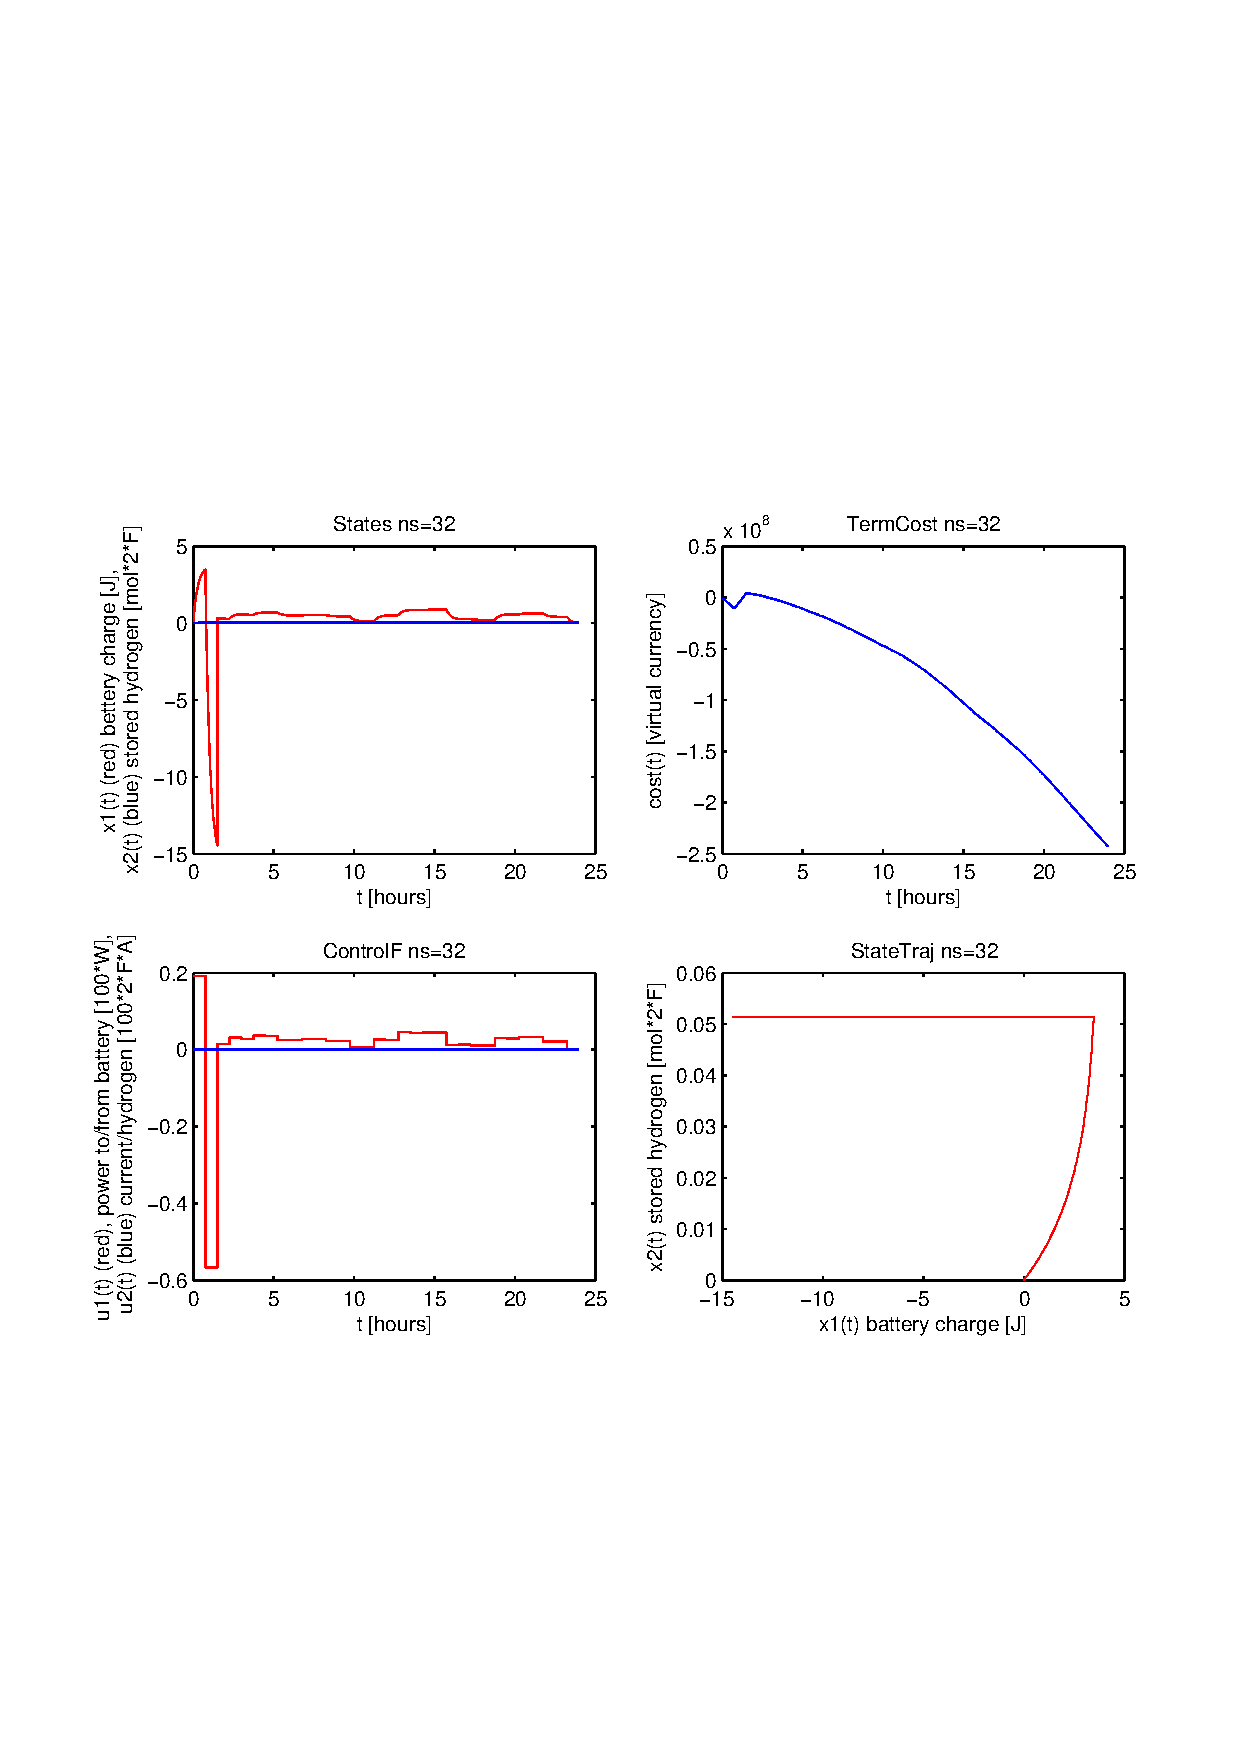
\includegraphics[width=0.9\textwidth]{Obrazky/matepsfigFILTERSD}\caption{\label{fig:Filtersd} FilterSD solver results.}
\end{figure}
\begin{figure}
\begin{centering}
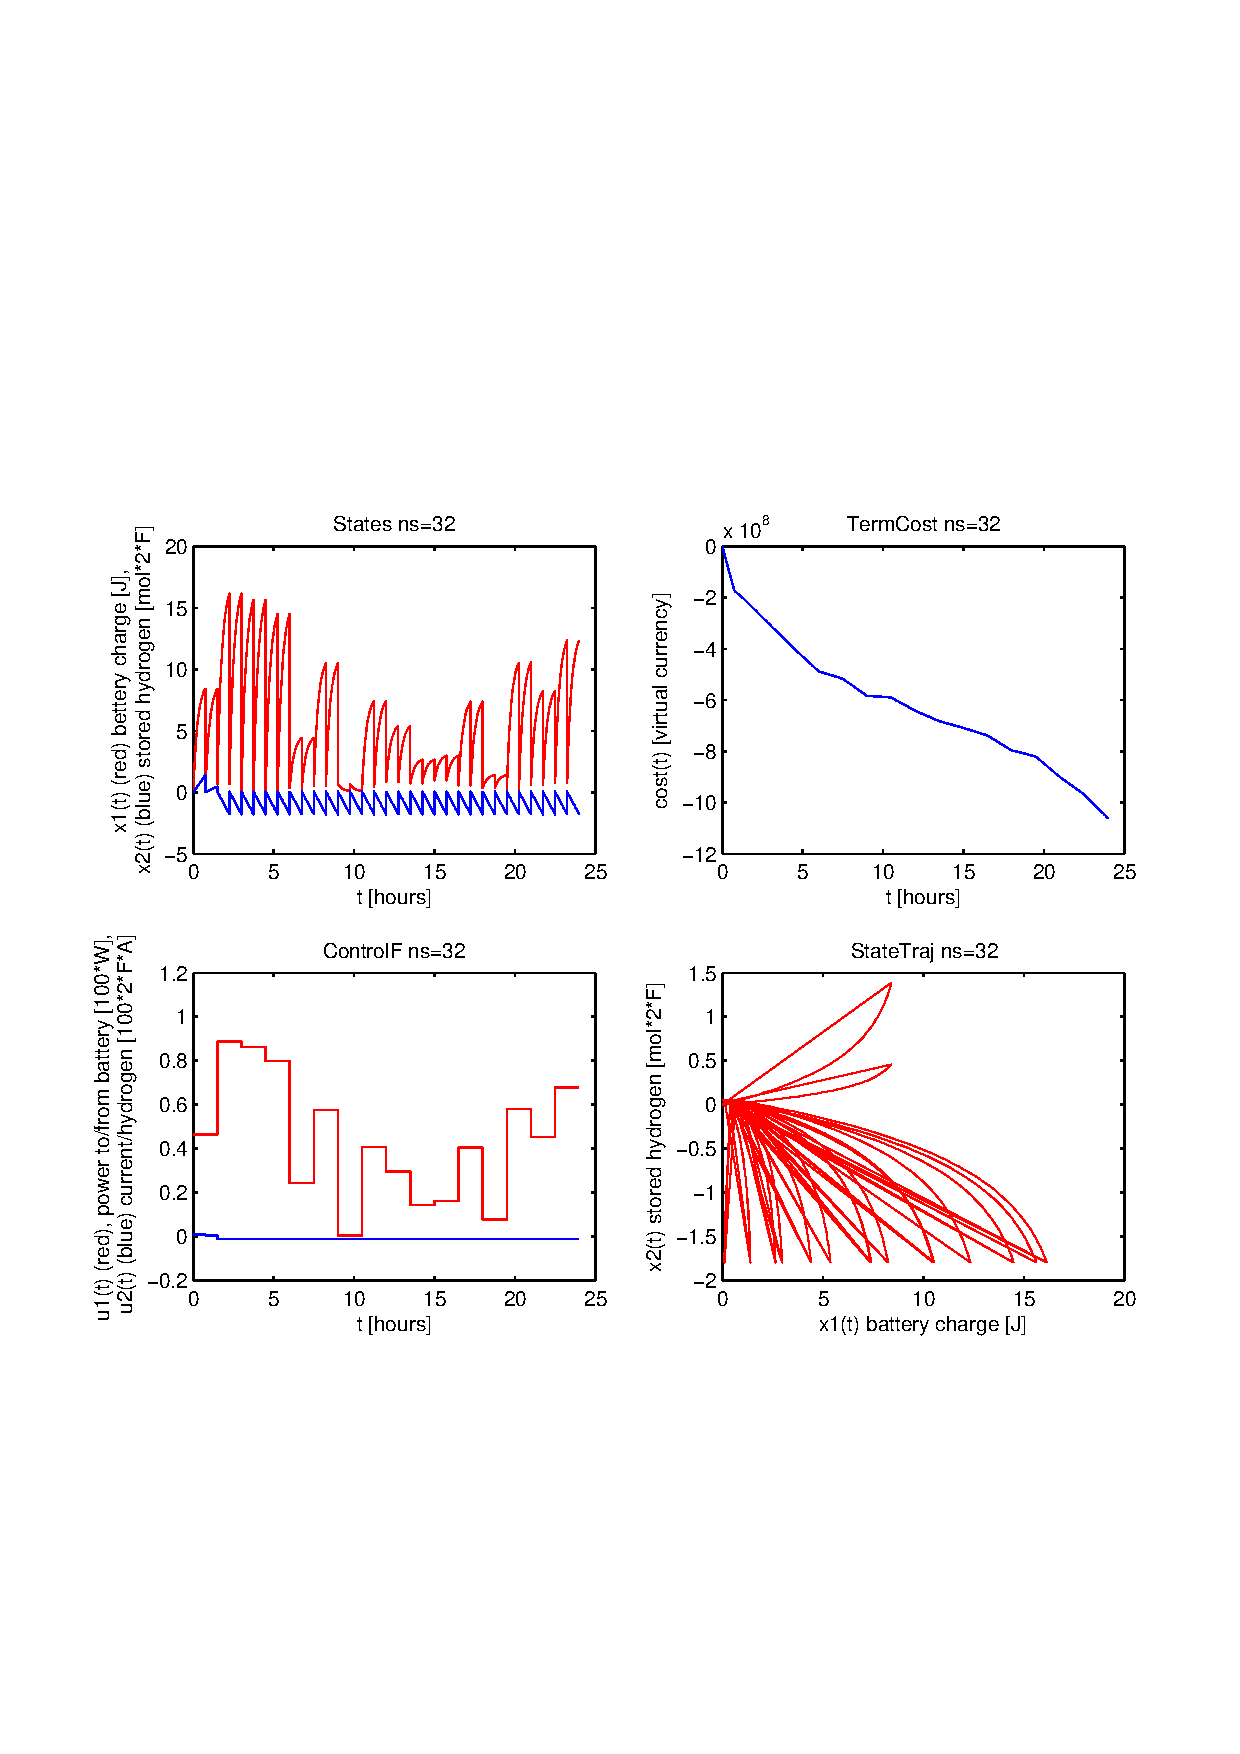
\includegraphics[width=0.9\textwidth]{Obrazky/matepsfigNLOPT}
\par\end{centering}

\caption{\label{fig:NLOPT}NLOPT solver results. Note that it did not manage
to satisfy the constraints.}
\end{figure}
\begin{figure}
\begin{centering}
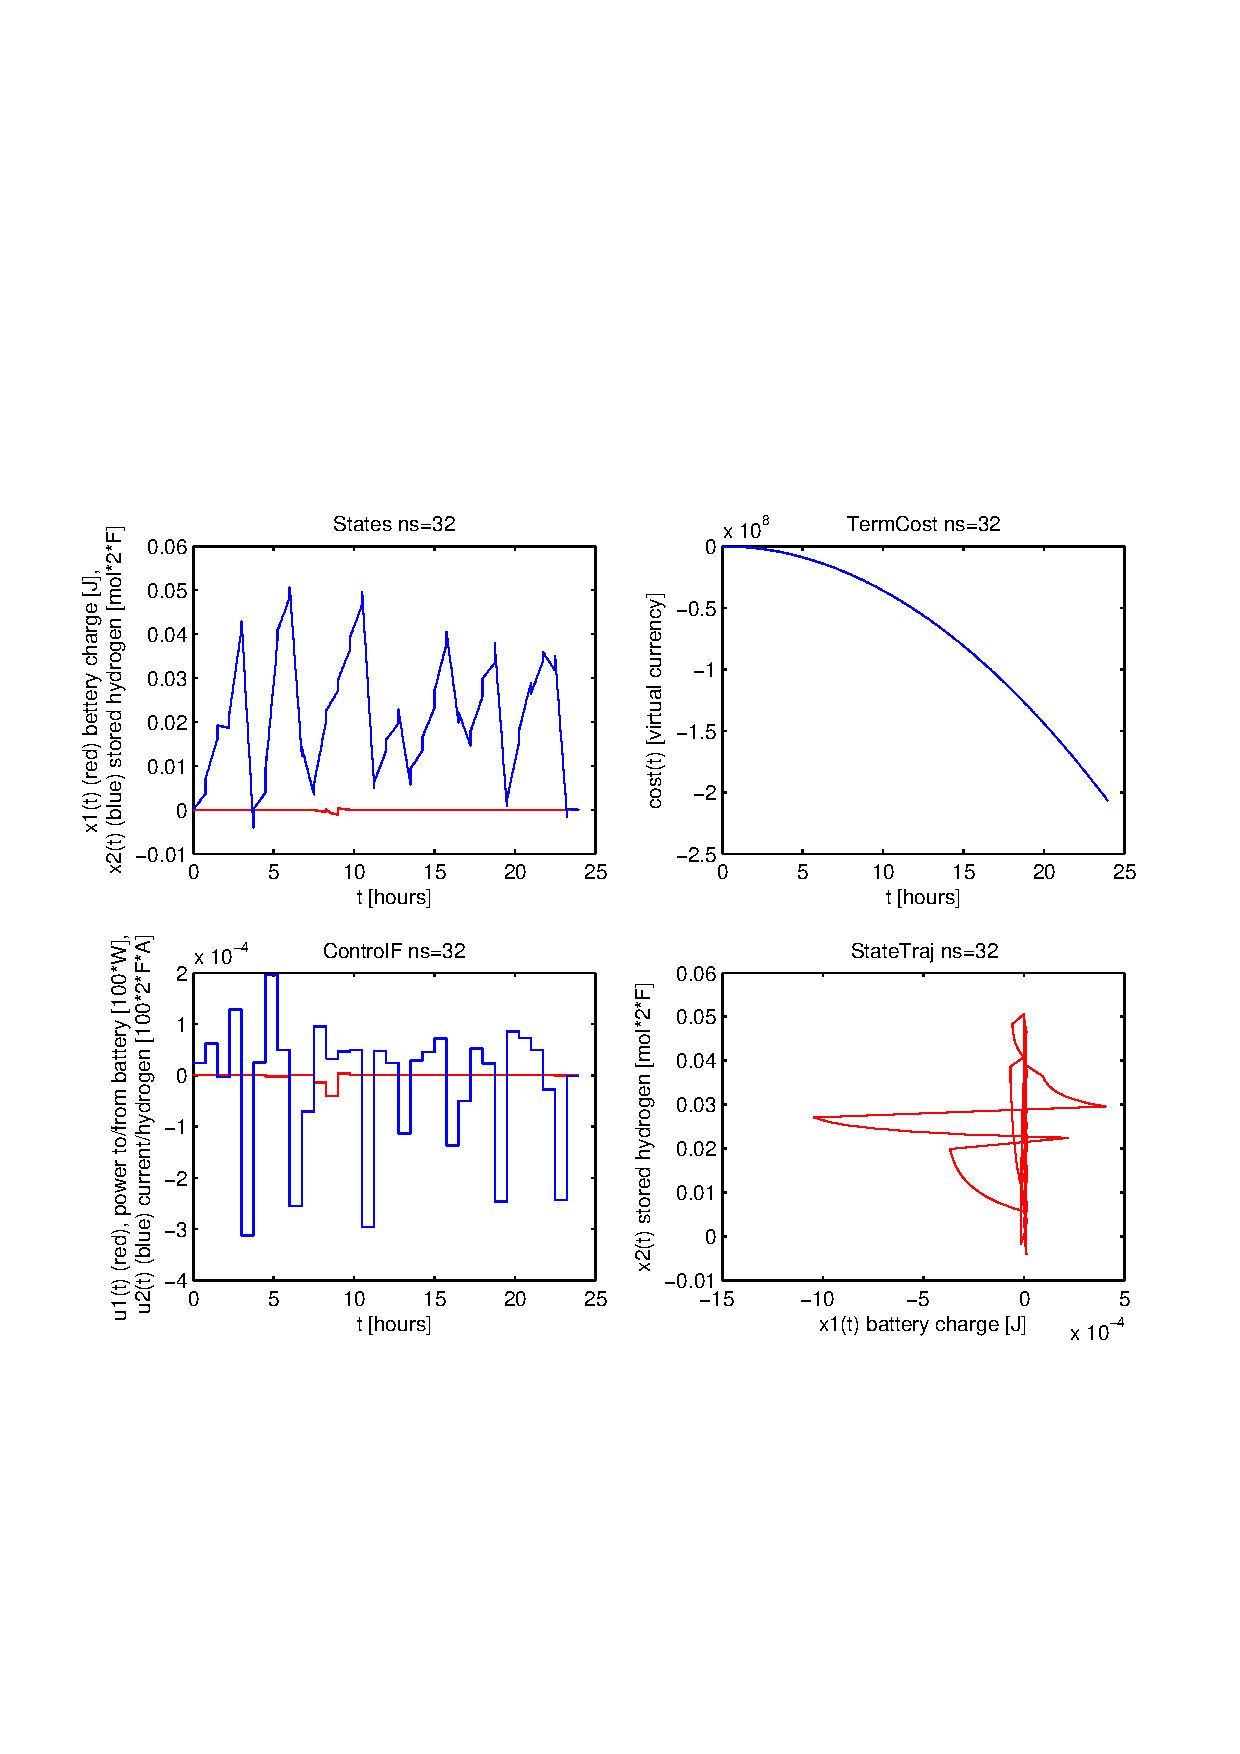
\includegraphics[width=0.9\textwidth]{Obrazky/matepsfigSQP}
\par\end{centering}

\caption{\label{fig:SQP}SQP Algorithm results}
\end{figure}



\subsection{Summary}

First, we have looked up optimal control and fuel cells works and
articles, including deeper links to existence results. Then, we have
applied a numerical optimal control method on a physical problem in
a way, so that we got:
\begin{itemize}
\item a new method for optimizing system (and system's cost) not against
a certain strategy, but against ideal maximum instead (which would
work even better in the need of additional control strategy change
in runtime).
\item a new method for comparing strategies against ideal maximum - to allow
to answer a question whether we can get better, that could not be
otherwise answered.
\item matlab implementation allowing for solver changes for testing different
minimum finding algorithms (in case of breakdowns)
\end{itemize}
From the numerical experiments, the solver SQP was veryfied to be
well suited for the problem.

Future work could include tuning the method for real applications
- the process would need to be implemented, for example, on a graphic
card or a computing cluster to be faster. Also given a reasonable
forecast of sunshine and power consumption, it could actually control
the system (by precalculating the control for the next week each specified
step in time), though this would need to be tested against other (currently
considered) best power managment strategies. (Using previous forecast
as a starting point could make the calculation even faster.)


\subsection*{}

\pagebreak{}\listoffigures
\addcontentsline{toc}{chapter}{List of Figures}

\pagebreak{}

\bibliographystyle{alpha}
\phantomsection\addcontentsline{toc}{chapter}{\bibname}\bibliography{bibdata}
%\def\bibname{Bibliography}
%\begin{thebibliography}{99}
%\addcontentsline{toc}{chapter}{\bibname}
%\bibliography{bibdata} 
%\end{thebibliography}
\end{document}
